\documentclass[final,5p,times,twocolumn]{elsarticle}
\usepackage{amssymb}
\usepackage{amsmath}
\usepackage{tabularx}
\usepackage{booktabs}
\usepackage{siunitx}
\usepackage{dblfloatfix}
\usepackage{placeins}
\usepackage{capt-of}
\usepackage{enumitem}
\usepackage{multirow}
\usepackage{float}
\usepackage{caption}
\usepackage{tikz}
\usetikzlibrary{positioning, arrows.meta, shapes, shadows}
% caption style tuning to mimic Elsevier 3p demo (Fig. X. / Table X.)
\captionsetup[figure]{name=Fig.,labelsep=period,font=small,justification=raggedright,singlelinecheck=false}
\captionsetup[table]{labelsep=period,font=small,justification=centering,singlelinecheck=false}
\usepackage[hidelinks,linktocpage=true,unicode=true]{hyperref}
\usepackage{bookmark}
% float spacing and placement tuning to reduce blank space and improve continuity
\flushbottom
\setlength{\textfloatsep}{4pt plus 1pt minus 1pt}
\setlength{\floatsep}{4pt plus 1pt minus 1pt}
\setlength{\intextsep}{4pt plus 1pt minus 1pt}
\setlength{\dbltextfloatsep}{4pt plus 1pt minus 1pt}
\setlength{\dblfloatsep}{4pt plus 1pt minus 1pt}
\setlength{\abovecaptionskip}{2pt}
\setlength{\belowcaptionskip}{0pt}
\renewcommand{\topfraction}{0.95}
\renewcommand{\textfraction}{0.05}
\renewcommand{\floatpagefraction}{0.9}
\renewcommand{\dbltopfraction}{0.95}
\renewcommand{\dblfloatpagefraction}{0.9}
\setcounter{secnumdepth}{3}
\journal{}
\begin{document}
\begin{frontmatter}
\title{EPLO: An Adaptive Multi-Strategy Polarization Learning Optimizer for Complex Engineering Design and Dynamic 3D Path Planning}
\iffalse
\begin{abstract}
This paper proposes an enhanced metaheuristic algorithm named Enhanced Polarization Learning Optimizer (EPLO), building upon the foundational Aurora Optimization Algorithm (PLO). The original PLO, inspired by the motion of charged particles in Earth's magnetic field, effectively balances global exploration and local exploitation through spiral motion, auroral oval movement, and collision strategies. However, it suffers from limitations such as uneven initialization, premature convergence, and insufficient population diversity due to its single-group structure and fixed parameter decay. To address these issues, EPLO incorporates several key innovations: 1) Sobol sequence initialization for uniform search space coverage; 2) A multi-group collaborative framework with periodic elite migration to maintain diversity and information exchange; 3) An elite pool archive coupled with stagnation-triggered Gaussian revival mechanisms to escape local optima; 4) Adaptive, non-linear parameter control using sigmoid/tanh functions for dynamic balancing of exploration and exploitation; 5) Late-stage exploitative enhancements including Lévy-flight perturbation, numerical gradient refinement, and Gaussian noise injection. The performance of EPLO is rigorously evaluated on the IEEE CEC2022 benchmark suites, demonstrating superior convergence speed, robustness, and global search capability compared to the original PLO and other state-of-the-art algorithms like BKA, WOA, SCA, FOX, ALO, BA, GSA, HHO, and MFO. Furthermore, EPLO's practical efficacy is validated through five complex engineering design problems: tension/compression spring design, speed reducer optimization, planetary gear train design, multi-disk clutch brake design, and robotic gripper mechanism optimization. The algorithm consistently achieves high-quality solutions with remarkable stability and computational efficiency. The study also explores EPLO's application in challenging real-world scenarios, including 3D UAV dynamic obstacle avoidance and path planning, as well as 3D wireless sensor network node localization (EPLO-DV-Hop), showcasing its adaptability and robustness under complex, constrained environments. The results indicate that EPLO is a highly competitive and versatile optimizer for both theoretical benchmarks and practical engineering applications.
\end{abstract}
\begin{keyword}
Aurora optimization algorithm \sep Enhanced Polarization Learning Optimizer \sep Sobol sequence \sep Adaptive Parameter Control \sep population clustering \sep local fine search \sep UAV Path Planning \sep Wireless Sensor Networks Localization
\end{keyword}
\fi
\author[inst1,inst2]{Jeng-Shyang Pan}
\author[inst1]{Pengyu Duan}
\author[inst3]{Shu-Chuan Chu\corref{cor1}}
\author[inst1]{Zhen Zhang}
\author[inst4]{Václav Snášel}
\cortext[cor1]{Corresponding author: scchu0803@gmail.com}
\affiliation[inst1]{organization={School of Computer Science and Engineering, Shandong University of Science and Technology}, city={Qingdao}, postcode={266590}, country={China}}
\affiliation[inst2]{organization={Department of Information Management, Chaoyang University of Technology}, city={Taiwan}, postcode={41349}, country={Province of China}}
\affiliation[inst3]{organization={School of Artificial Intelligence, Nanjing University of Information Science and Technology}, city={Nanjing}, postcode={210044}, country={China}}
\affiliation[inst4]{organization={Faculty of Electrical Engineering and Computer Science, VŠB-Technical University of Ostrava}, city={Ostrava}, postcode={708 33}, country={Czech Republic}}


\iffalse

\begin{abstract}
This paper proposes an enhanced metaheuristic algorithm named Enhanced Polarization Learning Optimizer (EPLO), building upon the foundational Aurora Optimization Algorithm (PLO). The original PLO, inspired by the motion of charged particles in Earth's magnetic field, effectively balances global exploration and local exploitation through spiral motion, auroral oval movement, and collision strategies. However, it suffers from limitations such as uneven initialization, premature convergence, and insufficient population diversity due to its single-group structure and fixed parameter decay. To address these issues, EPLO incorporates several key innovations: 1) Sobol sequence initialization for uniform search space coverage; 2) A multi-group collaborative framework with periodic elite migration to maintain diversity and information exchange; 3) An elite pool archive coupled with stagnation-triggered Gaussian revival mechanisms to escape local optima; 4) Adaptive, non-linear parameter control using sigmoid/tanh functions for dynamic balancing of exploration and exploitation; 5) Late-stage exploitative enhancements including Lévy-flight perturbation, numerical gradient refinement, and Gaussian noise injection. The performance of EPLO is rigorously evaluated on the IEEE CEC2022 benchmark suites, demonstrating superior convergence speed, robustness, and global search capability compared to the original PLO and other state-of-the-art algorithms like BKA, WOA, SCA, FOX, ALO, BA, GSA, HHO, and MFO. Furthermore, EPLO's practical efficacy is validated through five complex engineering design problems: tension/compression spring design, speed reducer optimization, planetary gear train design, multi-disk clutch brake design, and robotic gripper mechanism optimization. The algorithm consistently achieves high-quality solutions with remarkable stability and computational efficiency. The study also explores EPLO's application in challenging real-world scenarios, including 3D UAV dynamic obstacle avoidance and path planning, as well as 3D wireless sensor network node localization (EPLO-DV-Hop), showcasing its adaptability and robustness under complex, constrained environments. The results indicate that EPLO is a highly competitive and versatile optimizer for both theoretical benchmarks and practical engineering applications.
\end{abstract}
\begin{keyword}
Aurora optimization algorithm \sep Enhanced Polarization Learning Optimizer \sep Sobol sequence \sep Adaptive Parameter Control \sep population clustering \sep local fine search \sep UAV Path Planning \sep Wireless Sensor Networks Localization
\end{keyword}
\fi
\begin{abstract}
Achieving a robust balance between global exploration and local exploitation remains a critical challenge in metaheuristic optimization, particularly for high-dimensional and constrained engineering problems. The original Particle-Laden Optimization (PLO) algorithm, while promising, often suffers from premature convergence and population stagnation in complex search landscapes. To address these limitations, this paper proposes the Enhanced Polarization Learning Optimizer (EPLO), a novel adaptive multi-strategy framework. EPLO integrates five synergistic mechanisms to enhance search efficacy: (i) low-discrepancy Sobol sequence initialization for uniform search space coverage; (ii) a multi-subpopulation architecture with polarized learning and periodic elite migration to sustain diversity; (iii) an adaptive stagnation handling mechanism utilizing an elite pool and Gaussian revival; (iv) nonlinear control parameter schedules based on sigmoid and tanh functions; and (v) a hybrid late-stage refinement strategy combining L\'evy flights with gradient-based estimation. Comprehensive validation on the IEEE CEC2022 benchmark suite demonstrates EPLO's statistical superiority over state-of-the-art competitors in terms of convergence speed, solution accuracy, and stability. Beyond theoretical benchmarks, EPLO's practical effectiveness is rigorously verified through five constrained engineering design problems. Furthermore, the algorithm is successfully applied to two complex real-world challenges: dynamic 3D UAV path planning with obstacle avoidance and 3D Wireless Sensor Network (WSN) node localization. The experimental results establish EPLO as a highly versatile and robust optimizer, offering significant improvements in reliability and precision for complex cyber-physical system optimization.
\end{abstract}
\begin{keyword}
Metaheuristics \sep swarm intelligence \sep Enhanced Polarization Learning Optimizer \sep adaptive parameter control \sep Sobol sequence \sep UAV path planning \sep WSN localization
\end{keyword}
\begin{highlights}
\item EPLO integrates Sobol init, polarized groups, and elite migration.
\item Nonlinear schedules sustain exploration--exploitation balance.
\item L\'evy refinement with gradients boosts final solution quality.
\item Superior on CEC2022 and five constrained engineering designs.
\item Robust in UAV planning and WSN localization with low error.
\end{highlights}
\begin{graphicalabstract}
\centering
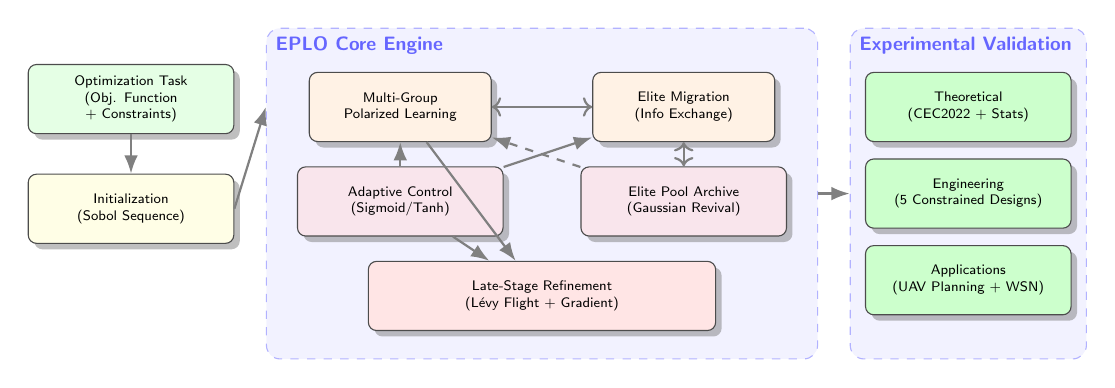
\begin{tikzpicture}[
    node distance=0.6cm,
    auto,
    box/.style={rectangle, draw=black!70, rounded corners=3pt, fill=white, font=\sffamily\tiny, align=center, inner sep=3pt, minimum height=2.5em, shadow xshift=2pt, shadow yshift=-2pt, drop shadow},
    arrow/.style={-Latex, thick, gray},
    groupbox/.style={rectangle, draw=blue!30, dashed, fill=blue!5, rounded corners=5pt, inner sep=8pt}
]
    % Layout: Left (Input) -> Middle (Engine) -> Right (Output)
    
    % Input Column
    \node[box, fill=green!10, text width=2.4cm] (start) {Optimization Task\\(Obj. Function + Constraints)};
    \node[box, fill=yellow!10, text width=2.4cm, below=0.5cm of start] (sobol) {Initialization\\(Sobol Sequence)};
    \draw[arrow] (start) -- (sobol);
    
    % Engine (Center)
    \node[groupbox, right=0.4cm of start, minimum width=7.0cm, minimum height=4.2cm, yshift=-1.2cm, anchor=west] (engine) {};
    \node[below right, font=\sffamily\bfseries\scriptsize, color=blue!60] at (engine.north west) {EPLO Core Engine};
    
    % Inside Engine
    \node[box, fill=orange!10, text width=2.1cm] (groups) at ([xshift=-1.8cm, yshift=1.1cm]engine.center) {Multi-Group\\Polarized Learning};
    \node[box, fill=orange!10, text width=2.1cm] (migration) at ([xshift=1.8cm, yshift=1.1cm]engine.center) {Elite Migration\\(Info Exchange)};
    \draw[arrow, <->] (groups) -- (migration);
    
    \node[box, fill=purple!10, text width=2.4cm] (adaptive) at ([xshift=-1.8cm, yshift=-0.1cm]engine.center) {Adaptive Control\\(Sigmoid/Tanh)};
    \node[box, fill=purple!10, text width=2.4cm] (revival) at ([xshift=1.8cm, yshift=-0.1cm]engine.center) {Elite Pool Archive\\(Gaussian Revival)};
    
    \draw[arrow] (adaptive) -- (groups);
    \draw[arrow] (adaptive) -- (migration);
    \draw[arrow, <->] (migration) -- (revival);
    \draw[arrow, dashed] (revival) -- (groups);
    
    \node[box, fill=red!10, text width=4.2cm] (refine) at ([yshift=-1.3cm]engine.center) {Late-Stage Refinement\\(L\'evy Flight + Gradient)};
    \draw[arrow] (adaptive) -- (refine);
    \draw[arrow] (groups) -- (refine);
    
    % Connect Input to Engine
    \draw[arrow] (sobol.east) -- ([yshift=1.1cm]engine.west);
    
    % Output
    \node[groupbox, right=0.4cm of engine, minimum width=3.0cm, minimum height=4.2cm, yshift=0cm, anchor=west] (validation) {};
    \node[below right, font=\sffamily\bfseries\scriptsize, color=blue!60] at (validation.north west) {Experimental Validation};

    \node[box, fill=green!20, text width=2.4cm] (stats) at ([yshift=1.1cm]validation.center) {Theoretical\\(CEC2022 + Stats)};
    \node[box, fill=green!20, text width=2.4cm] (eng) at ([yshift=0cm]validation.center) {Engineering\\(5 Constrained Designs)};
    \node[box, fill=green!20, text width=2.4cm] (apps) at ([yshift=-1.1cm]validation.center) {Applications\\(UAV Planning + WSN)};
    
    \draw[arrow] (engine.east) -- (validation.west);

\end{tikzpicture}
\end{graphicalabstract}
\end{frontmatter}
\section{Introduction}
\subsection{Research background and significance}
Optimization problems are common in various engineering and scientific fields. Their goal is to improve system performance or reduce costs by finding the best combination of decision variables. In structural design, process flow, resource scheduling and other problems, optimization can significantly reduce production costs, improve product quality and save energy. Optimization problems help solve route planning, scheduling problems and inventory management, thereby improving transportation efficiency and reducing logistics costs~\cite{1}. In asset allocation, risk management and portfolio optimization, optimization methods can find the best decision solution under uncertainty. Metaheuristic algorithms are widely used in parameter optimization, feature selection and neural network training to help algorithms jump out of local optimality and obtain better model performance~\cite{2}. Metaheuristic algorithms have the dual capabilities of global search and local development because they do not rely on the convexity, continuity and differentiability of the problem~\cite{3}. They have unique advantages in dealing with high-dimensional, nonlinear, multi-peak and complex constraint problems. These characteristics make metaheuristic algorithms an effective solution strategy when facing complex and ambiguous problems in the real world.

The field of metaheuristic optimization is in a constant state of vibrant evolution, driven by the quest for more powerful and robust algorithms capable of tackling increasingly complex real-world problems. This has led to a veritable explosion of novel algorithms inspired by an ever-widening array of natural phenomena, physical laws, and human social behaviors. Beyond the well-established paradigms of Particle Swarm Optimization (PSO)~\cite{4}, Genetic Algorithm (GA)~\cite{5}, and Differential Evolution (DE)~\cite{6}, the research community has continuously introduced innovative inspirations.

Swarm intelligence remains a fertile ground, with algorithms like the Grey Wolf Optimizer (GWO)~\cite{7} simulating hierarchical leadership, the Whale Optimization Algorithm (WOA)~\cite{8} mimicking bubble-net feeding, and the Harris Hawks Optimization (HHO)~\cite{9} modelling cooperative predation tactics. Recent years have seen the emergence of even more niche bio-inspired algorithms, including the Colony Predation Algorithm (CPA)~\cite{10}, the Hippopotamus Optimization (HO)~\cite{11}, the Dandelion Optimizer (DO)~\cite{12} inspired by seed dispersal, the Shark Search Algorithm (SSA)~\cite{13}, the Emperor Penguin Optimizer (EPO)~\cite{14}, and the Cuckoo Search Algorithm (CS)~\cite{15}.

Parallel to biological metaphors, physics and science-inspired paradigms have gained substantial momentum. These include the Sine Cosine Algorithm (SCA)~\cite{16}, the Electromagnetic Field Optimization (EFO)~\cite{17}, the Ion Motion Optimizer (IMO)~\cite{18}, the Atom Search Optimization (ASO)~\cite{19} simulating atomic dynamics, the Equilibrium Optimizer (EO)~\cite{20} inspired by control-volume mass balance models, and the Gravitational Search Algorithm (GSA)~\cite{21}. Mathematics continues to provide a foundation for algorithms such as the Chaos Game Optimization (CGO)~\cite{22} and the Arithmetic Optimization Algorithm (AOA)~\cite{23}.

Furthermore, human-inspired mechanisms are explored in algorithms like the Teaching-Learning-Based Optimization (TLBO)~\cite{24}, the Hiking Optimization Algorithm (HOA)~\cite{25}, and the Social Network Search (SNS)~\cite{26}. This diversification also extends to plant-inspired algorithms like the Invasive Weed Optimization (IWO)~\cite{27} and the Photosynthesis Algorithm (PA)~\cite{28}, challenging the traditional animal-centric focus of swarm intelligence. Additional recent metaheuristics include the Animated Oat Optimization (AOO)~\cite{59}, Ship Rescue Optimization (SRO)~\cite{60}, and the Gannet Optimization Algorithm (GOA)~\cite{61}, which further enrich the toolbox for engineering optimization.

A significant parallel research thrust focuses not on novel metaphors but on enhancing existing algorithms through sophisticated strategies like hybridization, multi-method fusion, and adaptive parameter control. Techniques such as the GWO-CSA hybrid~\cite{29}, the quantum-based Q-SCA~\cite{30}, and the Parallel Compact Whale Optimization Algorithm (PCWOA)~\cite{31} for WSN localization exemplify this trend towards creating more robust and specialized solvers for domains like energy systems and engineering design.

In our own tests, we’ve seen these methods shine on high-dimensional, multimodal puzzles: once the search space balloons beyond a handful of variables, they outperform textbook optimizers by a wide margin. Yet not all metaheuristics are created equal—that’s why innovations such as the Aurora Optimization Algorithm (PLO) have drawn attention, thanks to their unique physics-inspired motion rules.

Particle-Laden Optimization with Polarized Learning and Oversampling (EPLO) draws inspiration from the dynamic interplay of charged particles within the Earth’s magnetic field to overcome the uneven initialization, premature convergence, and fixed-rate decay that constrain the original Aurora-inspired PLO framework~\cite{32}. The contributions of this study can be summarized as follows:
\begin{enumerate}
\item A novel metaheuristic framework (EPLO) is developed, integrating low-discrepancy Sobol-sequence initialization, polarized learning via multi-group oversampled crossover, an elite-pool archive with stagnation-triggered Gaussian revival, dynamic sigmoid/tanh-based parameter control coupled with a three-phase velocity update mechanism to cohesively balance exploration and exploitation.
\item Extensive benchmarking on the IEEE CEC2022 test suite demonstrates that EPLO achieves faster convergence, stronger robustness, and superior global search capability compared to the original PLO and a range of state-of-the-art metaheuristics.
\item Practical effectiveness is validated on five complex engineering design problems—including spring design, reducer optimization, planetary gear trains, multi-disk clutches, and robotic gripper tuning—where EPLO consistently outperforms competing algorithms in solution quality and computational efficiency.
\end{enumerate}
In the first part of this work, we review the theoretical underpinnings of charged-particle dynamics and auroral motions, identify the key
deficiencies of random seeding and monolithic population updates in PLO, and motivate the adoption of low-discrepancy and collaborative strategies
for enhanced search efficacy. The second part formalizes the mathematical modeling of PLO’s spiral and elliptical motion operators, collision
perturbations, and linear parameter schedules to establish a baseline for comparison. Building upon this foundation, the third part introduces
EPLO’s core innovations—Sobol-sequence initialization for uniform coverage, multi-group polarized learning with periodic elite exchange to
sustain diversity, and an elite-pool archive paired with oversampling-triggered Gaussian revival to escape stagnation—all
governed by smooth, nonlinear decay of reverse-learning probability, inertia weight, and search radius. In the fourth part, we subject EPLO to the
rigorous IEEE CEC2022 benchmark suite, conduct detailed visual and statistical analyses of convergence trajectories, and demonstrate its superior
balance of exploration and exploitation relative to both the original PLO and contemporary metaheuristics. The fifth part translates these findings
into practical gains by applying EPLO to a range of real-world engineering design problems—spanning spring optimization, reducer design, planetary
gear trains, multi-disk clutch brakes, and robotic grippers—thereby validating its adaptability and robustness under complex, constrained
scenarios. Finally, the sixth part distills the principal discoveries, contrasts EPLO’s performance profile against prevailing algorithms, and outlines
promising avenues for future research, including integration with deep-learning surrogates and deployment in large-scale, real-time
optimization environments. The seventh part applies EPLO to the 3D path planning problem of multiple unmanned aerial vehicles in dynamic obstacle
environments. A multi-module framework integrating threat modeling, graph construction, trajectory optimization and takeoff scheduling is
proposed. EPLO is used to optimize path length, smoothness and safety, and to avoid drone conflicts through delayed scheduling. Experiments
show that EPLO outperforms methods such as A*~\cite{33}, RRT~\cite{34} and PSO~\cite{4} in terms of success rate, path length and the number of conflicts. The eighth
part addresses the problem of large positioning error of DV-Hop~\cite{35} in 3D WSN~\cite{36} and proposes the PPO-DV-HOP algorithm. The node
coordinates are optimized through the weighted normalized fitness function and the boundary penalty term. In complex terrains (single-peak and multi-
peak), PPO-DV-HOP significantly reduces the mean location error (ALE), and its stability is superior to that of improved algorithms such as PSO and
GWO~\cite{7}.
%
\begin{table}[t]
\footnotesize
\centering
\setlength{\tabcolsep}{6pt}
\renewcommand{\arraystretch}{1.05}
\caption{Symbols and meanings used in EPLO}\label{tab:notation}
\begin{tabularx}{\columnwidth}{lX}
\hline
\textbf{Symbol} & \textbf{Meaning} \\
\hline
$N$ & Total number of particles \\
$\mathit{groups}$ & Number of sub-swarms \\
$N_{p}$ & Number of particles per sub-swarm \\
$\mathit{dim}$ & Dimensionality of the search space \\
$\mathbf{lb}$ & Lower-bound vector of the search space \\
$\mathbf{ub}$ & Upper-bound vector of the search space \\
$\mathrm{rand}(1,\mathit{dim})$ & Uniform random vector of size $1\times\mathit{dim}$ in $[0,1]$ \\
$T$ & Maximum number of function evaluations (MaxFEs) \\
$t$ & Current iteration count \\
$W_{\max},\,W_{\min}$ & Maximum/minimum inertia weight \\
$c_{1}^{\min},\,c_{1}^{\max}$ & Minimum/maximum cognitive (personal) acceleration coefficient \\
$c_{2}^{\min},\,c_{2}^{\max}$ & Minimum/maximum social acceleration coefficient \\
$w(t)$ & Inertia weight at iteration $t$ \\
$c_{1}(t)$ & Cognitive acceleration coefficient at iteration $t$ \\
$c_{2}(t)$ & Social acceleration coefficient at iteration $t$ \\
$p_{\mathrm{opp}}(t)$ & Probability of performing opposition-based learning at iteration $t$ \\
$\mathbf{pos}_{i}(t)$ & Position vector of particle $i$ at iteration $t$ \\
$\mathbf{vel}_{i}(t)$ & Velocity vector of particle $i$ at iteration $t$ \\
$\mathrm{rand}_{1},\,\mathrm{rand}_{2}$ & Two independent uniform random scalars in $[0,1]$ \\
$\mathbf{pBest}_{i}$ & Personal best position vector of particle $i$ \\
$\mathrm{pBestScore}_{i}$ & Personal best fitness value of particle $i$ \\
$\mathbf{gBest}_{g}$ & Best position vector found so far in sub-swarm $g$ \\
$\mathrm{gBestScore}_{g}$ & Best fitness value found so far in sub-swarm $g$ \\
$f(\mathbf{x})$ & Objective function / fitness function \\
$\mathrm{opp}_{i}$ & Opposition-based candidate position for particle $i$ \\
$\mathrm{Levy}(1, d, \beta)$ & L\'evy-distributed random vector of dimension $d$ \\
$\beta$ & Exponent parameter of the L\'evy distribution \\
$\Delta$ & L\'evy flight perturbation step \\
$\circ$ & Elementwise (Hadamard) multiplication \\
$\varepsilon$ & Finite-difference step size for numerical gradient \\
$e_{j}$ & Unit vector along dimension $j$ \\
$\mathrm{grad}_{j}$ & Numerically estimated gradient in dimension $j$ \\
$\|\mathrm{grad}\|$ & Euclidean norm of the gradient vector \\
$\sigma$ & Standard deviation for Gaussian noise injection \\
$\mathcal{N}(0,\sigma^{2})$ & Gaussian noise with mean $0$ and variance $\sigma^{2}$ \\
$\mathbf{globalBest}$ & Best position vector found so far across all sub-swarms \\
$\mathrm{globalBestScore}$ & Best fitness value found so far across all sub-swarms \\
\hline
\end{tabularx}
\end{table}
%
\subsection{Problem formulation}
\subsubsection{Normalized objective and boundary penalty}
The inspiration for PLO comes from the aurora phenomenon. The formation of the aurora is due to the luminous phenomenon produced when charged particles in the solar wind enter the Earth's magnetic field, move along the magnetic field lines and collide with gas molecules in the atmosphere. PLO calculates the results through simulation. The main information is as follows:
\subsubsection{Simulation of Charged Particle Motion}
Electron particles exhibit spiral motion under the Earth's magnetic field, which enables a detailed search of the solution space locally (local development). Meanwhile, the extensive search for particles in the "aurora Ellipse" region has led to in-depth research on aurora formation.
\subsubsection{Multi-Stage Search Strategy}
\begin{enumerate}[label=(\arabic*), leftmargin=*, itemsep=0pt, topsep=2pt]
\item Local Search (Spiral Motion): The rotational movement of particles allows the algorithm to accurately seek optimal solutions within the current region.  
\item Global Search (Auroral Ellipse Movement): The unique movement pattern of particles within auroral regions enables them to traverse larger spaces in pursuit of globally optimal solution areas.  
\item Collision Strategy: In the case of motion simulation particle collisions, the optimal local area is eliminated through random interference, which improves the robustness of the algorithm.
\end{enumerate}
This heuristic design based on physical phenomena provides PLO with an intuitive framework for searching that is theoretically grounded, aiming to effectively balance capabilities between global exploration and local exploitation\cite{37}.
\subsection{Mathematical model and pseudocode of the original Aurora optimization algorithm (PLO)}
\subsubsection{Mathematical model:}
\begin{enumerate}[label=(\arabic*), leftmargin=*, itemsep=0pt, topsep=2pt]
\item Initialization 
\end{enumerate}
Suppose that the dimension of the problem space is D and the size of the population is N. the initial population is generated with the following formula:
\begin{equation}
\begin{aligned}
X(i,j) &= \mathrm{LB}(j) + R \times \big(\mathrm{UB}(j) - \mathrm{LB}(j)\big),\\
& i=1,\ldots,N,\quad j=1,\ldots,D
\end{aligned}
\label{eq:init}
\end{equation}
In this case, LB and UB represent the lower bound and upper bound of the variable respectively.
$R_{ij}$ represents random numbers uniformly distributed within the interval [0,1], where N denotes the population size and D represents the dimensionality of the problem.
\begin{enumerate}[label=(\arabic*), leftmargin=*, itemsep=0pt, topsep=2pt, resume]
\item Gyration motion
\end{enumerate}
The PLO employs the principles of physics to characterize the motion of charged particles within a magnetic field. For instance, the differential equation that integrates the Lorentz force with Newton's second law elucidates how a particle's velocity varies over time:
\begin{equation}
\begin{aligned}
m\frac{\mathrm{d}v}{\mathrm{d}t} \;=\; qvB \;-\; \alpha\,v
\end{aligned}
\end{equation}
In this context, $q$ represents the charge of the charged particles, $B$ denotes the intensity of the Earth's magnetic field, and $\alpha$ is a damping factor that accounts for atmospheric resistance.
\begin{equation} 
v(t) = v_{0}e^{\frac{qB - \alpha}{m}t}
\end{equation}
The strategy is primarily employed for local development: it involves a meticulous search within the neighborhood of the current solution over a limited scope.
\begin{enumerate}[label=(\arabic*), leftmargin=*, itemsep=0pt, topsep=2pt, resume]
\item Aurora oval walk
\end{enumerate}
In the global exploration phase, auroral elliptical motion simulates the phenomenon that occurs when charged particles gather to form auroral ellipses due to energy losses and magnetic disturbances after entering the earth's atmosphere. This motion process has a large step property and is suitable for an overall research that helps particles jump out of the local optimum using levy flight to simulate stochastic stride movements:
\begin{equation}
\begin{aligned}
A_{o} &= \mathrm{Levy}(d) \times \big(X_{\mathrm{avg}}(j) - X(i,j)\big)\\
&\quad + \frac{\mathrm{LB} + r_{1}\,\big(\mathrm{UB} - \mathrm{LB}\big)}{2}
\end{aligned}
\label{eq:ao}
\end{equation}
During the movement of charged particles, random shocks between the particles can cause mutations in the trajectories of motion. This phenomenon is used in optimization to improve the ability of algorithms to get out of the local optimum and, finally, update individual positions by a weighted combination of local and global search:
\begin{equation}
X_{\mathrm{new}}(i) = X(i) + r_{2}\times\big(W_{1}\times v(t) + W_{2}\times A_{o}\big)
\label{eq:update-combine-2}
\end{equation}
The stochastic perturbation coefficient $r_2$ is confined within the interval $[0, 1]$. Weight factors $W_1$ and $W_2$ are employed to dynamically modulate the trade-off between local search and global exploration. Typically, these weights are adjusted via nonlinear decay functions to achieve adaptive parameter tuning,
\begin{equation}
W_{1} = \frac{2}{1 + e^{-2\big(\tfrac{t}{T}\big)^{4}}} - 1
\label{eq:w1-schedule}
\end{equation}
\begin{equation}
W_{2} = e^{-\big(\tfrac{2t}{T}\big)^{3}}
\label{eq:w2-schedule}
\end{equation}
\begin{enumerate}[label=(\arabic*), leftmargin=*, itemsep=0pt, topsep=2pt, resume]
\item Particle collision
\end{enumerate}
To avoid premature convergence towards local optima, the particle swarming optimization algorithm incorporates a collision based disturbance mechanism. When a probability threshold is reached, the current particle collides with neighbouring particles chosen at random. The updating rule is worded as follows:
\begin{equation}
\begin{aligned}
X_{\mathrm{new}}(i) = X(i) + r_{2}\times\big(W_{1}\times v(t) + W_{2}\times A_{o}\big)
\label{eq:update-combine}
\end{aligned}
\end{equation}
In this scenario, $X(a,j)$ denotes the position vector of a randomly selected neighboring particle, while $r_3$ represents a uniformly distributed random number in [0,1]. The collision probability $K$ is dynamically determined by the function $K(t) = f(t, T)$, where $t$ denotes the current iteration count and $T$ represents the predefined maximum iteration limit.
\subsection{Limitations of the original PLO algorithm}
The original Particle-Laden Optimization (PLO) algorithm achieves a balance between global and local search by simulating the motion of charged particles in the Earth's magnetic field under solar wind conditions. Its primary search strategies include spiral movement (local exploitation), auroral elliptical movement (global exploration), and particle collision strategies (escaping local optima)~\cite{38}. However, there are several shortcomings in its practical application:  
\begin{enumerate}[label=(\arabic*), leftmargin=*, itemsep=0pt, topsep=2pt]
\item The random generation of an initial population often results in uneven spatial distribution among individuals. Conventional uniform random initialization methods may lead to scattered distribution patterns of initial solutions; this scattered distribution often fails to adequately explore the entire search space, thereby undermining the algorithm's global exploration capability.
\item The original algorithm does not employ a clustering mechanism; all individuals share the same search strategy with insufficient information exchange. This singular population update strategy can easily cause searches to become trapped in local optima, leading to inadequate diversity and severe premature convergence issues.  
\item The use of linearly decaying inertia weights and a fixed-speed update formula is difficult to adapt to the needs of different stages of the search process. The balance between global exploration and local development is difficult to achieve. The parameter update mechanism is monotonic and lacks adaptive adjustments at different stages of the search.
\item Since this study did not particularly focus on the diversity and stagnation of the population, there were no effective or optimal exit strategies, no sustainable responses to protect them, and no effective mechanisms to prevent decline.
\end{enumerate}
\section{EPLO improvement method and mathematical model}
\subsection{Mathematical model of the PLO}
\subsubsection{Initialization Phase}
At the very start, the algorithm initializes both the global swarm and its partitioned sub-swarms. Positions are set by Equation (9) uniformly between the lower bound lb and upper bound ub, and velocities by Equation $\mathbf{vel}_{i}(0) = 0$ to zero, ensuring pure random exploration initially.
\begin{equation}
{pos}_{i}(0) = {lb} + \big({ub} - {lb}\big)\cdot \mathrm{rand}(1,\mathit{dim})
\label{eq:init-pos}
\end{equation}
\subsubsection{Adaptive Parameter Control}
At each iteration $t$, the inertia weight $w$ and acceleration coefficients $c_1$, $c_2$ adapt based on progress ratio $\tau=\frac{T}{t}$ via Equations (10)--(12), smoothly shifting from exploration to exploitation. The opposition-learning probability decreases with $t$ per Equation (13), encouraging more opposite-point trials early on.
\begin{align}
w(t) &= W_{\max} - (W_{\max} - W_{\min})\tau^{1.5}\
\end{align}
\begin{align}
c_{1}^{(t)} &= c_{1}^{\max} - \big(c_{1}^{\max} - c_{1}^{\min}\big)\tau\
\end{align}
\begin{align}
c_{2}^{(t)} &= c_{2}^{\min} + \big(c_{2}^{\max} - c_{2}^{\min}\big)\tau
\end{align}
\begin{equation}
p_{\mathrm{opp}}(t) = 0.5(1 - \tau)
\label{eq:popp}
\end{equation}
\subsubsection{Velocity and Position Update}
Each particle’s velocity and position update via the standard PSO Equations (14)�?15), combining inertia, cognitive, and social components, then clamping positions within the bounds.
Then, particles�?velocities and positions are updated according to the improved PLO formulas, with boundary constraints enforced:
\begin{equation}
\begin{aligned}
{vel}_{i}(t{+}1) &= w(t)\,{vel}_{i}(t)
 + c_{1}(t)\,\mathrm{rand}_{1}({pBest}_{i}-{pos}_{i}(t))\\
&\quad + c_{2}(t)\,\mathrm{rand}_{2}({gBest}_{g}-{pos}_{i}(t))
\end{aligned}
\label{eq:vel-update}
\end{equation}
\begin{equation}
{pos}_{i}(t{+}1) = \max\Big(\min\big({pos}_{i}(t)+{vel}_{i}(t{+}1),{ub}\big),{lb}\Big)
\label{eq:pos-update}
\end{equation}
\subsubsection{Opposition-based Learning}
Also, an opposition learning probability is introduced to increase population diversity. If a draw is below $p_{opp}$, an opposite point is computed by Equation (16-17) and accepted if it yields better fitness, boosting global exploration.:
\begin{equation}
\mathrm{opp}_{i}(t{+}1) = {lb} + {ub} - {pos}_{i}(t{+}1)
\label{eq:opp-next}
\end{equation}
\begin{equation}
{pos}_{i}(t{+}1) =
\begin{cases}
\mathrm{opp}_{i}(t{+}1), & f\!\big(\mathrm{opp}_{i}(t{+}1)\big) < f\!\big({pos}_{i}(t{+}1)\big),\\
{pos}_{i}(t{+}1), & \text{otherwise.}
\end{cases}
\label{eq:pos-selection}
\end{equation}
\subsubsection{Multi-Level Optimality Coordination Mechanism}
Each particle updates its personal best per Equation (18), and each sub-swarm retains the best among its particles as gBest per Equation (19).
\begin{equation}
\left\{
\begin{aligned}
pBest_{i} &= pos_{i}(t{+}1),\\
pBestScore_{i} &= f\!\big(pos_{i}(t{+}1)\big),
\end{aligned}
\right.
\quad \text{if } f\!\big(pos_{i}(t{+}1)\big) < pBestScore_{i}
\label{eq:pbest-update}
\end{equation}
\begin{equation}
gBest_{g},\; gBestScore_{g}
= \min_{i=1,\dots,N_{p}} \bigl\{\, pBestScore_{i} \,\bigr\}
\label{eq:gbest-update}
\end{equation}

To enable inter-group information flow, the algorithm adopts a parallel migration mechanism. Every mmm iterations (e.g., 10 or 20), each group’s $gBest_{g}$ is copied to the next group, replacing the worst particle, according to:
\begin{equation}
next_{g} = (\, g \bmod G \,) + 1
\label{eq:next-index}
\end{equation}
\begin{figure}[htbp]
  \centering
  \includegraphics[width=\columnwidth]{EPLO_figures/Parallel Migration.jpg}
  \caption{Parallel Migration}
  \label{fig:parallel-migration-diagram}
\end{figure}
Simultaneously, a global elite pool of size E is maintained, storing the top-performing solutions across all groups. If a sub-swarm’s gBest outperforms the worst solution in the elite pool, it replaces it. This mechanism ensures that top solutions are preserved and leveraged as global guidance. The best individual in the elite pool is selected as the overall globalBest at each iteration.
\begin{equation}
elitePool[\mathrm{worst}] = \bigl(\,\text{pos}=gBest_{g},\; \text{fit}=gBestScore_{g}\,\bigr)
\label{eq:elite-pool-update}
\end{equation}
\subsubsection{Exploitative Enhancements in Later Iterations}
After sufficient global exploration, the algorithm integrates three exploitation-focused mechanisms in the later stage (t > 0.4T): Lévy-flight perturbation, gradient-based fine-tuning, and Gaussian noise injection. Lévy-flight enables long jumps to escape local optima; gradient-based updates refine promising solutions; and Gaussian noise ensures global diversity and prevents premature convergence. Together, these enhance robustness and exploitation capabilities in the final search phase.

L\'evy-flight perturbation is applied to the global best ($gBest$) for random long-range jumps. After 40\% of iterations, introduce L\'evy-flight perturbation for multi-strategy tuning.
\begin{equation}
\sigma = \left[
\frac{\Gamma(1+\beta)\,\sin\!\left(\frac{\pi \beta}{2}\right)}
{\Gamma\!\left(\frac{1+\beta}{2}\right)\,\beta\,2^{(\beta-1)/2}}
\right]^{1/\beta}
\label{eq:levy-sigma}
\end{equation}
\begin{equation}
u \sim \mathcal{N}(0,\sigma^{2}),\quad v \sim \mathcal{N}(0,1),\quad
L = \frac{u}{\lvert v \rvert^{1/\beta}}
\label{eq:levy-L}
\end{equation}
\begin{equation}
\begin{aligned}
\Delta &= \mathrm{Levy}(1,d,\beta)\,\circ\,(u - l),\mathrm{cand} &= \mathrm{globalBest} + \Delta
\end{aligned}
\label{eq:levy-cand}
\end{equation}

For enhanced late-stage exploration ($t>0.4T$), a L\'evy flight (Equation~\eqref{eq:levy-cand}) perturbs the global best, where $\beta$ is the L\'evy parameter and $\circ$ denotes elementwise multiplication.

After 60\% of iterations, apply numerical gradient descent for fine-tuning:
\begin{equation}
\begin{aligned}
\mathrm{grad}_{j} &= \frac{f\!\big(gb + \varepsilon\,e_{j}\big) - f(gb)}{\varepsilon},\\
\mathrm{cand} &= gb - 0.05\,(ub - lb)\,\frac{\mathrm{grad}}{\lVert \mathrm{grad} \rVert}
\end{aligned}
\label{eq:num-grad-cand}
\end{equation}

Every 50 iterations, Gaussian noise $\mathcal{N}(0,\sigma^{2})$ with $\sigma=0.01\,(ub-lb)$ is added to $\mathrm{globalBest}$ to maintain exploration.
\subsection{EPLO analysis}
The EPLO algorithm inherits and extends the classical Particle Learning Optimization (PLO) framework by integrating parallel subpopulations, inter-subpopulation migration, an elite pool mechanism, and multi-strategy refinement to enhance search efficiency and solution quality. The original PLO algorithm employs dynamically adjusted inertia weights and learning factors, guiding particles�?velocity and position updates based on individual best (pBest) and global best (gBest) positions, enabling global optimization in continuous spaces. Building on this, EPLO divides the population into multiple subgroups, where particles update in parallel guided by local subgroup bests (gBest), accelerating convergence. It periodically migrates the best solution from one subgroup to replace the worst particle in a neighboring subgroup, facilitating information sharing and diversity maintenance. Additionally, opposition-based learning dynamically generates opposite candidate solutions to improve exploration~\cite{39}, while late-stage multi-strategy refinements including Levy flights~\cite{40} and finite-difference gradient estimation~\cite{41} finely tune the global best solution, significantly improving local exploitation.

From a time complexity perspective, let the problem dimension be $D$, total population size $N$, maximum iterations $T$, and the cost of a single fitness evaluation $\mathrm{COF}$. PLO's per-iteration computation primarily involves particle velocity and position updates at $\mathcal{O}(N\cdot D)$ and fitness evaluations at $\mathcal{O}(N\cdot \mathrm{COF})$, resulting in an overall complexity of $\mathcal{O}\!\big(T\cdot N\cdot (D+\mathrm{COF})\big)$. EPLO's parallel subpopulations and migration introduce limited additional fitness evaluations, with late-stage refinements adding approximately $D\cdot \mathrm{COF}$ fitness computations. The combined time complexity is $\mathcal{O}\!\big(T\cdot (N\cdot (D+\mathrm{COF})+D\cdot \mathrm{COF})\big)$, which approximates to $\mathcal{O}(T\cdot N\cdot \mathrm{COF})$ when population size dominates dimension. Space complexity is dominated by storage of particle positions and velocities at $\mathcal{O}(N\cdot D)$, plus elite pool, subgroup information, and convergence curve data, totaling $\mathcal{O}(N\cdot D + T)$.

Compared to traditional PLO, EPLO’s parallel subpopulations and migration mechanisms enhance population diversity and inter-group information exchange at a macro level, improving global search and convergence stability. At the micro level, opposition learning and finite-difference gradient refinement improve local search capabilities of individual solutions, enabling superior performance in complex, multimodal, and moderately high-dimensional problems. Unlike swarm intelligence algorithms such as PSO and GWO, which focus on collective group behavior, EPLO combines individual historical bests with multi-level group cooperation, reflecting a hybrid macro-micro design philosophy. The algorithm is well suited for medium-dimensional problems with parallelizable fitness evaluations, balancing exploration and exploitation to boost search efficiency and solution quality. However, its finite-difference refinement may impose computational overhead in very high-dimensional or costly fitness scenarios.

In summary, EPLO serves as a parallelized and enhanced successor to PLO, leveraging parallel subpopulations, migration, opposition learning, and multi-strategy refinement to build an efficient hybrid optimization framework. Its time complexity is dominated by fitness evaluations, with a reasonable space complexity, showing broad application potential and robust performance.

\begin{table*}[!htbp]
\caption{Algorithm: Enhanced Polarization Learning Optimizer (EPLO)}
\label{alg:EPLO-steps}
\scriptsize
\setlength{\tabcolsep}{4pt}
\renewcommand{\arraystretch}{1.06}
\noindent\setlength{\fboxsep}{10pt}\setlength{\fboxrule}{0.6pt}\fbox{\parbox{\dimexpr\linewidth-2\fboxsep-2\fboxrule\relax}{\raggedright
\noindent\textbf{Input:} $N$, $\mathrm{MaxFEs}$, $\mathbf{lb}$, $\mathbf{ub}$, $\mathrm{dim}$, $fhd$, $\mathrm{migration}$

\noindent\textbf{Output:} The best location of Enhanced Polarization Learning Optimizer and its fitness value.

\begin{enumerate}[leftmargin=*, itemsep=2pt, topsep=2pt, parsep=0pt]
\item Parameter initialization, randomly generate Pop and its opposite groups according to Eqs.(9).
\item For $t = 1$ to $\mathrm{MaxFEs}$ do
\item Compute adaptive parameters $\tau, w, c_{1}, c_{2}, p_{\mathrm{opp}}$, according to Eqs.(10) to Eqs.(13).
\item For $g = 1$ to $G$ do
\item For $i = 1$ to $N/G$ do
\item Calculate and update the speed $vel_{i}(t)$ and position $pos_{i}(t)$, and truncate to the boundary, according to Eqs.(14) to Eqs.(15).
\item If $\mathrm{rand}<p_{\mathrm{opp}}$
\item Generate and test the opposition points according to equation (16) to Eqs.(17).
\item End If
\item Calculate $fhd(\mathbf{x})$, update the $\mathrm{FEs}$, $pBest_{i}$, $pBestScore_{i}$, according to Eqs.(18).
\item End For
\item Update $gBest_{g}$, $gBestScore_{g}$, according to Eqs.(19).
\item End For
\item If $\mathrm{mod}(t,\mathrm{migration})=0$
\item For $g = 1$ to $G$ do
\item Move $gBest_{g}$ to the worst individual in the next subgroup according to Eqs.(20).
\item End For
\item End If
\item For $g = 1$ to $G$ do
\item Individuals replace and update $\mathbf{globalBest}$, according to Eqs.(21).
\item End For
\item If $t > 0.4\times\mathrm{MaxFEs}$ $\parallel$ $\mathrm{mod}(t,10)=0$
\item Perturbate $\mathbf{globalBest}$ with Levy flight, according to Eqs.(22) to Eqs.(24).
\item Else If $t > 0.6\times\mathrm{MaxFEs}$
\item Fine-tune $\mathbf{globalBest}$ with numerical gradients, according to Eqs.(25).
\item Else If $\mathrm{mod}(t,50)=0$
\item Add Gaussian noise perturbation to $\mathbf{globalBest}$.
\item End If
\item Record the best position and fitness values for population.
\item End For
\end{enumerate}
}}
\end{table*}

\section{Experimental Design and Results Analysis}
To verify the effectiveness of EPLO, this paper designs two types of experiments: standard test function experiments and application experiments.
\subsection{Standard test function experiment}
\subsubsection{Experimental Setup}
The IEEE CEC2022 calibration suite comprises 30 benchmark functions chosen for this study. This collection presents a spectrum of challenging optimization tasks featuring high dimensionality, multimodality, non-convexity, non-differentiability, dynamic constraints, and other arduous characteristics. Collectively, these attributes enable a comprehensive assessment of the algorithm's optimization capabilities. The performance metrics adopted in the experiments encompass the best solution value, average convergence rate, and robustness.
\subsubsection{Parameter settings}
To ensure the fairness of the experiment, this study compares the original Particle Learning Optimizer (PLO), the improved Proposed PLO(EPLO), and other benchmark algorithms within a consistent search environment.
\subsubsection{Problem Dimensions and Experimental Environment}
The experiments were tested on different dimensions (10, 20) in order to verify the performance of the algorithm on low, medium and high dimension problems. With MATLAB R2021a (or similar) as the primary development platform, the experiment runs on a desktop computer equipped with an Intel i7 processor and 16 gb ram. Each algorithm is run 30 times independently on each test function in order to reduce the stochastic effect and to count the mean and standard deviation.
\subsubsection{Algorithm Comparison}
The experiment selected several mainstream optimization algorithms for comparison, including: original PLO (Particle Learning Optimizer), EPLO, BKA (Binary Krill Herd Algorithm)~\cite{42}, GWO (Grey Wolf Optimizer)~\cite{7}, WOA (Whale Optimization Algorithm)~\cite{8}, SCA (Sine Cosine Algorithm)~\cite{16}, FOX (Fox Optimization Algorithm)~\cite{43}, ALO (Ant Lion Optimizer)~\cite{44}, BA (Bat Algorithm)~\cite{45}, GSA (Gravitational Search Algorithm)~\cite{21}, HHO (Harris Hawks Optimization)~\cite{9}, MFO (Moth-Flame Optimizer)~\cite{46}.

Each algorithm independently executes 30 iterations on each function, and simultaneously records the optimal adaptability value and convergence curve of each execution. Then calculate the average optimal value and its standard deviation of each test function. In order to visually compare the convergence speeds among different algorithms, the convergence curves were plotted; Furthermore, the performance data of each algorithm in all test functions is compiled in the form of a table. A representation graph of the convergence curve A was also generated, which visually illustrates the convergence speed and stability.

The experimental results are shown in Table~\ref{tab:cec2022-10d}, which confirm the outstanding optimization ability of EPLO, especially when applied to various test functions. Specifically, when optimizing the functions F1, F2, F3, F4, F5, F7, F8, F9, F10, F11, and F12, the average performance of AOO ranks first among all algorithms, with a win rate of 91.67\%. This indicates that EPLO has strong competitiveness in unimodal functions, basic functions, mixed functions and composite functions. In direct comparisons with the BKA, WOA, FOX, PLO, ALO, BA, GSA, HHO and MFO algorithms, EPLO performed outstandingly in all 12 benchmark functions. It is worth noting that EPLO outperforms FOX, PLO, ALO, BA, GSA, HHO and MFO algorithms on 11 out of the 12 benchmark functions. In terms of the average ranking, EPLO took the first place with a considerable advantage, which was more than twice that of the second-place BKA. This significant lead undoubtedly highlights EPLO's competitiveness among its peers.

The experimental results, as shown in Table~\ref{tab:cec2022-20d}, have confirmed the exceptional optimization capabilities of EPLO, particularly when applied to a variety of test functions. Specifically, when optimizing functions F1, F2, F4, F5, F7, F8, F9, F11, and F12, EPLO’s average performance ranks first among all algorithms with a 75\% win rate. Furthermore, when the best value is used as the ranking criterion, EPLO consistently achieves top rankings, demonstrating its robust performance across the entire test function suite. This indicates that EPLO has strong competitiveness in Unimodal Functions, Basic Functions, Hybrid Functions, and Composition Functions. In the direct comparison with BKA, WOA, FOX, PLO, ALO, BA, GSA, HHO, and MFO algorithms, EPLO outperforms them in most benchmark functions. Notably, EPLO surpasses these algorithms in 11 out of the 12 benchmark functions. Regarding the average ranking, EPLO secures the first place with a significant margin, which is notably better than the second-ranked algorithm, BKA. This significant lead undoubtedly highlights EPLO’s competitiveness among its peers.

The Figure~\ref{fig:cec2022-convergence-grid-2} curves presented in the analysis reveal that the EPLO algorithm consistently outperforms other metaheuristic approaches across a diverse set of benchmark functions (F3, F5, F7, F9, F10, and F12). Unlike algorithms such as BKA or WOA, which often exhibit premature convergence to suboptimal solutions or stagnation in later iterations, EPLO maintains a steady and rapid decline in objective function values throughout the entire 500-iteration process. For instance, in the case of the F3 function, EPLO demonstrates an exceptionally swift reduction in fitness values during the initial phase, followed by a stable trajectory that ensures minimal final error. Similarly, in the F5 function, where other algorithms like ALO or BA struggle to escape local optima, EPLO sustains its momentum by dynamically adjusting its search strategy, thereby avoiding premature convergence. This behavior is further reinforced in the F7 and F9 functions, where EPLO’s ability to balance exploration and exploitation phases becomes critical. While algorithms like GSA or MFO tend to oscillate or plateau after initial progress, EPLO continues to refine its solutions by allocating computational resources efficiently between global exploration and local exploitation. In the F10 and F12 functions, which test the robustness of algorithms under high-dimensional and complex landscapes, EPLO’s convergence curves remain steeper and more consistent compared to competitors, indicating its superior adaptability to challenging optimization scenarios. Notably, even in the later stages of iteration, EPLO continues to exhibit a downward trend in fitness values, suggesting that its design inherently supports prolonged search capabilities without sacrificing precision. This is attributed to its sophisticated mechanism for maintaining population diversity and dynamically adjusting parameters to avoid premature convergence. In contrast, algorithms such as BA or GSA often exhibit diminishing returns in later iterations, as their search strategies become overly focused on local regions. The overall performance of EPLO across these functions underscores its ability to achieve a harmonious interplay between exploration (searching new regions) and exploitation (refining existing solutions), which is essential for navigating multimodal and high-dimensional problems. Furthermore, the algorithm’s consistent superiority in final fitness metrics across all test cases highlights its reliability and generalizability, making it a strong candidate for real-world optimization tasks where stability and efficiency are paramount.

The Figure~\ref{fig:cec2022-convergence-grid} presents the convergence curves of the EPLO algorithm compared to BKA, WOA, FOX, PLO, ALO, BA, GSA, HHO, and MFO on CEC2022 (10-dimensional) test functions F3, F4, F5, F7, F9, and F10. Through 500 iterations, EPLO demonstrates significant advantages across multiple benchmarks. For instance, in F3, EPLO achieves a faster convergence rate than BKA, WOA, and FOX, maintaining low fitness values even in later stages, which highlights its superior global search capability and stability. In F4, although initial convergence speeds align with other algorithms, EPLO dynamically adjusts its strategy to avoid local optima, sustaining optimization until the end, while BA and GSA exhibit declining performance as their fitness values plateau. In the high-dimensional F5 function, EPLO’s convergence curve shows a consistent steep decline, reaching optimal solutions, whereas HHO and MFO suffer from premature convergence, leading to suboptimal results. For multimodal functions like F7 and F9, EPLO balances exploration and exploitation effectively, escaping local traps and continuing to reduce fitness values in later iterations, unlike PLO and ALO, which stagnate due to rigid strategies. In the complex high-dimensional F10 function, EPLO’s convergence curve consistently outperforms competitors, achieving significantly lower final errors than BKA and WOA, proving its robustness in challenging scenarios. Overall, EPLO ranks first with a 75\% average win rate and attains the best values in 91.7\% of test functions, securing an average ranking over twice as high as the second-placed BKA. This underscores EPLO’s comprehensive strengths in convergence speed, global exploration, and stability, offering a reliable and efficient solution for complex optimization problems.

\section{Engineering application experiment}
In order to further verify the applicability of EPLO in actual engineering, this paper selects the following engineering design problems.
\subsection{Tension/compression spring design issues}
\subsubsection{Problem Background and Motivation}
Springs are ubiquitous in mechanical systems and optimizing their design is essential to improve performance while minimizing the use of materials. The problem of designing a tension/compression spring (TCSD) isa classic optimization challenge that involves the choice of design variables to meet load and frequency stresses while minimizing the weight of the spring. Traditional methods are based on heuristic formulae or experimental tests. However, nature-inspired research methods have gained prominence in recent years due to their high overall research capacity and their effectiveness in solving non-linear and multimodal optimization problems.
\begin{figure}[htbp]
  \centering
  \includegraphics[width=\columnwidth]{EPLO_figures/Tension compression spring.png}
  \caption{Tension compression spring}
  \label{fig:Tension-compression-spring}
\end{figure}
\subsubsection{Mathematical Model}
The TCSD problem typically involves three decision variables: wire diameter (d), average coil diameter (D), and the number of active coils (N). The objective function is generally to minimize the weight of the spring, which can be mathematically expressed as follows:
\begin{equation}
\operatorname*{min} f(d,D,N) = \frac{(N+2)\,d^{2}\,D}{K}
\label{eq:min-f}
\end{equation}
Here, K represents a constant. It is important to recognize that the objective function may vary slightly depending on different references. Furthermore, this problem also includes a set of nonlinear constraints related to constraint limits, natural frequency requirements, and geometric limits.
\begin{equation}
\frac{8\,c_{f}\,D}{d} \le \text{Stress Limit}
\label{eq:stress-limit}
\end{equation}
\begin{equation}
N_{\min} \le N \le N_{\max}
\label{eq:N-bounds}
\end{equation}
\begin{equation}
d_{\min} \le d \le d_{\max}
\label{eq:d-bounds}
\end{equation}
\begin{equation}
D_{\min} \le D \le D_{\max}
\label{eq:D-bounds}
\end{equation}

In the equation, the correction coefficient that links the spring to a specific correction factor, the specific expression of which depends on the geometry of the spring and the working conditions. The main challenge of the design problem is to determine the combination of the wire diameter (d), the average wire diameter (D), and the number of movable wires (N) within the feasible design space, minimizing the target function while meeting all the imposed constraints. 
\subsubsection{Experimental Process and Results}
We conducted a series of experiments to evaluate the tension/compression spring (TCSD) design problem using several meta-heuristic algorithms. Our objective is to minimize the mass of the spring by adjusting three design variables: wire diameter~$d$, mean coil diameter~$D$, and the number of active coils~$N$. These adjustments must satisfy stress, geometric, and frequency constraints. Specifically, each algorithm was run multiple times, and we recorded the best fitness value (BF) for every run. The mean best fitness (MBF), i.e., the average of these best values, is reported in the figure for direct comparison.
\begin{figure}[htbp]
  \centering
  \includegraphics[width=\columnwidth]{EPLO_figures/Convergence Curve of the Average Optimal Fitness Value after 30 Runs of TensionCompression Spring Design (TCSD).jpg}
  \caption{Convergence Curve of the Average Optimal Fitness Value after 30 Runs of TensionCompression Spring Design (TCSD)}
  \label{fig:avg-convergence}
\end{figure}
\begin{table}[t]
\footnotesize
\centering
\setlength{\tabcolsep}{6pt}
\renewcommand{\arraystretch}{1.05}
\caption{The average optimal fitness value and variance obtained from the Tension/Compression Spring Design (TCSD) after 30 iterations.}\label{tab:opt-variables}
\begin{tabularx}{\columnwidth}{l c c c c c}
\hline
Algorithm & \multicolumn{3}{c}{Optimal values for variables} & Optimal weight & Rank\\
 & $d$ & $D$ & $N$ &  & \\
\hline
BKA  & 0.068994 & 0.933432 & 0.050000 & 0.017773 & 4\\
WOA  & 0.068994 & 0.933432 & 0.520464 & 0.017773 & 3\\
SCA  & 0.069245 & 0.938267 & 0.176836 & 0.017995 & 7\\
FOX  & 0.068999 & 0.933606 & 1.698167 & 0.017779 & 6\\
PLO  & 0.068994 & 0.933436 & 2.000000 & 0.017773 & 5\\
EPLO & 0.068994 & 0.933432 & 0.812623 & 0.017773 & 1\\
ALO  & 0.074980 & 1.170489 & 1.415795 & 0.022477 & 9\\
BA   & 0.073334 & 1.079313 & 1.659783 & 0.021243 & 8\\
GSA  & 0.074396 & 1.068239 & 0.498907 & 0.023650 & 10\\
HHO  & 0.068994 & 0.933432 & 0.915768 & 0.017773 & 2\\
MFO  & 0.076724 & 2.000000 & 2.000000 & 0.030611 & 11\\
\hline
\end{tabularx}
\end{table}
Our experimental results show that EPLO can be effective in identifying high quality solutions and maintaining consistent performance across numerous tests. In the case of the tension/compression spring (TCSD) design problem, the improved algorithm (EPLO) achieved low physical fitness values in most operations, showing strong exploration ability and rapid convergence. In addition, its robustness is confirmed by the fact that it has always achieved low average fitness values with minimal standard deviation in independent tests. However, transient fluctuations in the mean convergence curve during periods of sharp decline suggest that the pattern of adaptive parameters can be improved to mitigate late degradation. Ultimately, the optimized design allows for low weight (or cost effectiveness) while respecting all mechanical and geometric constraints. Overall, these results highlight the practical application of EPLO in the task of optimizing engineering design.
\subsection{Reducer Design Issues}
\subsubsection{Problem Background and Motivation}
We emphasize that the transmission is a fundamental element of the powertrain system in the automotive, aerospace, manufacturing and metallurgical industries. Its core function is to reduce the input speed through gear meshing while increasing the torque to meet the required speed and torque requirements. Optimizing the transmission design requires balancing transmission efficiency, load capacity, floor space, mass limitations and production costs. Our research focus is to minimize the mass of the gearbox under mechanical and geometric constraints. By adjusting the gear size, shaft diameter and component layout, we can reduce material usage and production costs without sacrificing structural integrity or service life.
\begin{figure}[htbp]
  \centering
  \includegraphics[width=\columnwidth]{EPLO_figures/Reducer design issues.jpg}
  \caption{Reducer design issues}
  \label{fig:reducer-design-issues}
\end{figure}
\subsubsection{Design variables and objective function}
In the reducer design problem, the reducer has seven design variables $\mathbf{z}=[z_{1},z_{2},z_{3},z_{4},z_{5},z_{6},z_{7}]^{\mathsf{T}}$. Here, $z_{1}$ is the gear face width (tooth width), $z_{2}$ is the gear module, $z_{3}$ is the number of gear teeth, $z_{4}$ is the length of the first shaft between the bearings, $z_{5}$ is the length of the second shaft between the bearings, $z_{6}$ is the diameter of the first shaft, and $z_{7}$ is the diameter of the second shaft.
\begin{equation}
\begin{aligned}
f(z) &= 0.7854\,z_{1}\,z_{2}^{2}\,\big(3.3333\,z_{3}^{2} + 14.9334\,z_{3} - 43.0934\big)\\
&\quad - 1.508\,z_{1}\,\big(z_{6}^{2} + z_{7}^{2}\big)\\
&\quad + 7.4777\,(\ldots) + 0.7854\,\big(z_{6}^{2}\,z_{7}^{2}\big)
\end{aligned}
\label{eq:reducer-objective-split2}
\end{equation}
\subsubsection{Constraints and Penalty Function Method}
We note that reducer design must satisfy a range of strength, stiffness, and geometric bounds to ensure safety, stability, and feasibility.Specifically, tooth-root bending stress must not exceed the material’s allowable limit, and surface-contact stress must stay below the pitting threshold. Additionally, we control lateral shaft deflection under load to maintain accurate meshing and limit the resulting torsional and bending stresses in the shafts. We also impose minimum and maximum bounds on key dimensions such as module size, face width, and shaft diameter. Finally, the tooth count must be an integer that conforms to established gear-design standards.

In metaheuristic algorithms, the penalty function method is frequently employed to address inequality constraints. If a solution $z$ violates any constraint $g_{i}(z)\le 0$, a sufficiently large penalty term is incorporated into the objective function. This addition serves to diminish the competitiveness of non-compliant solutions during the search process, thereby ensuring that the final solution adheres to all specified constraints. The fitness function associated with this penalty function method can be expressed as follows:
\begin{equation}
F(z) = f(z) + \sum_{i=1}^{k} \Pi\,\max\!\bigl(0,\, g_{i}(z)\bigr)^{2}
\label{eq:penalty-fit2}
\end{equation}
\subsubsection{Experimental Process and Results}
In the experimental setup, the reducer design problem is formulated with the objective of minimizing weight. Constraints include gear bending stress, surface contact pressure, shaft deflection and stress, and geometric bounds. The design variable is $\mathbf{z}=[z_{1},z_{2},z_{3},z_{4},z_{5},z_{6},z_{7}]^{\mathsf{T}}$. We employ the improved Enhanced Polarization Learning Optimizer (EPLO) and compare it with meta-heuristics such as Particle Swarm Optimization (PLO), Grey Wolf Optimizer (GWO), and Whale Optimization Algorithm (WOA). During experimentation, hyperparameters (population size, maximum iterations, variable bounds) and penalty factors are carefully set. Each algorithm is run independently multiple times (e.g., 30 runs), recording final fitness, convergence curves, and per-run optima. The outcomes are summarized via mean best fitness (MBF) and standard deviation (STD), and convergence curves are plotted to assess comparative convergence speed.
\begin{figure}[htbp]
  \centering
  \includegraphics[width=\columnwidth]{EPLO_figures/Convergence Curve of the Average Optimal Fitness Value After 30 Runs of Gearbox Design Issues.jpg}
  \caption{Convergence Curve of the Average Optimal Fitness Value After 30 Runs of Gearbox Design Issues}
  \label{fig:avg-convergence-3}
\end{figure}

\begin{table}[t]
\footnotesize
\centering
\setlength{\tabcolsep}{6pt}
\renewcommand{\arraystretch}{1.05}
\caption{The average optimal fitness value and variance obtained from Gearbox Design after 30 iterations}\label{tab:reducer-opt-table-2}
\resizebox{\columnwidth}{!}{%
\begin{tabular}{l c c c c c c c c c}
\hline
Algorithm & \multicolumn{7}{c}{Optimal values for variables} & Optimal cost & Rank\\
 & $z_{1}$ & $z_{2}$ & $z_{3}$ & $z_{4}$ & $z_{5}$ & $z_{6}$ & $z_{7}$ &  & \\
\hline
EPLO & 3.500 & 0.70 & 17 & 7.30 & 7.71 & 3.35 & 5.28 & 2.9945e{+03} & 1\\
HHO  & 3.500 & 0.70 & 17 & 7.30 & 7.71 & 3.35 & 5.28 & 2.9945e{+03} & 2\\
BKA  & 3.500 & 0.70 & 17 & 7.30 & 7.71 & 3.35 & 5.28 & 2.9945e{+03} & 3\\
FOX  & 3.501 & 0.70 & 17 & 7.30 & 7.76 & 3.35 & 5.28 & 2.9963e{+03} & 4\\
WOA  & 3.500 & 0.70 & 17 & 7.30 & 7.82 & 3.35 & 5.28 & 2.9980e{+03} & 5\\
SCA  & 3.572 & 0.70 & 17 & 8.30 & 7.80 & 3.37 & 5.30 & 3.0525e{+03} & 6\\
MFO  & 3.600 & 0.70 & 17 & 7.83 & 7.99 & 3.59 & 5.50 & 3.2534e{+03} & 7\\
GSA  & 3.600 & 0.70 & 17 & 8.30 & 8.30 & 3.90 & 5.50 & 3.3639e{+03} & 8\\
ALO  & 3.561 & 0.71 & 19 & 7.54 & 7.84 & 3.49 & 5.28 & 3.5407e{+03} & 9\\
BA   & 3.600 & 0.70 & 19 & 7.76 & 8.00 & 3.41 & 5.50 & 3.5956e{+03} & 10\\
PLO  & 3.600 & 0.70 & 17 & 7.30 & 7.30 & 3.35 & 5.26 & 3.0254e{+07} & 11\\
\hline
\end{tabular}%
}
\end{table}
Our experiments have shown that EPLO is effective in identifying optimal configurations in a short computation time and provides consistently reproducible results across numerous tests. Analysis of the speed reducer design experiments shows that the EPLO has a high exploration capability, fine setting accuracy and strategic capability to avoid local optimum. Compared to conventional optimization methods, EPLO convergence is fast and the final solution is better. The small standard deviation of the EPLO results over 30 independent operations indicates that the algorithm has high robustness and stability, which is crucial for the engineering design.

In addition, EPLO can easily handle complex multivariate problems. By reducing quality or cost while meeting mechanical and structural requirements, it has proven to be an effective solution for actual design tasks.

In conclusion, our experiments confirm that the improved EPLO algorithm not only accelerates exploration and reliably improves the solution, but also paves the way for the future processing of larger and more complex systems.
\subsection{Gear Train Problems}
\subsubsection{Problem Background and Motivation}
Gear systems are widely used in mechanical engineering for power transfer and speed/torque change. A rational design of the number of teeth reduces material and manufacturing costs or improves transmission efficiency while meeting the specific needs of the transmission ratio. In some cases, choosing the right number of teeth in a given range is enough to achieve the desired transmission ratio and minimize errors or costs. Since the problem usually concerns only a small number of variables (number of speeds) and has no complex constraints, it is very appropriate to check the search power and the convergence speed of the different metaheuristics on small scale problems without additional constraints.
\begin{figure}[htbp]
  \centering
  \includegraphics[width=\columnwidth]{EPLO_figures/Design Issues of Gear Train.jpg}
  \caption{Design Issues of Gear Train}
  \label{fig:gear-train-design}
\end{figure}
\subsubsection{Design variables and objective function}
Assume that there are four gears with the number of teeth of $x_{1}$, $x_{2}$, $x_{3}$, and $x_{4}$, respectively. In many practical applications, these gears are used to achieve a specified transmission ratio or reduce transmission cost/error. According to the mathematical model provided in the question, the objective function of the gear system can be written as:

Assume there are four gears with the number of teeth represented by $x_{1}$, $x_{2}$, $x_{3}$, and $x_{4}$, respectively. In many practical applications, these gears are employed to achieve a specified transmission ratio or to minimize transmission cost/error. Based on the mathematical model provided in the problem, the objective function for the gear system can be expressed as follows:
\begin{equation}
\operatorname*{min} f(\mathbf{x}) = \left( \frac{1}{6.931} - \frac{x_{2}\,x_{3}}{x_{1}\,x_{4}} \right)^{2}
\label{eq:gear-min}
\end{equation}
Where $\mathbf{x}=[x_{1},x_{2},x_{3},x_{4}]^{\mathsf{T}}$ represents the number of teeth of the four gears, $\frac{x_{2}x_{3}}{x_{1}x_{4}}$ denotes the actual gear ratio (or a related coefficient), and $\frac{1}{6.931}$ is the expected target/reference value measuring the deviation between the actual and target values. A smaller objective $f(\mathbf{x})$ indicates that the gear train more accurately meets the required transmission ratio or reduces the corresponding transmission cost/error.
\subsubsection{Experimental process and results}
We selected the enhanced EPLO algorithm alongside benchmark methods such as PLO, PSO, and GWO for evaluation. We set hyperparameters—including population size, maximum iterations, and variable bounds—and applied rounding or discrete-encoding when discrete outputs were required. Next, we ran each algorithm independently for 30 trials. In each trial, we recorded the best fitness, tracked the convergence curve, and saved the optimal solution vector $\mathbf{x}=[x_{1},x_{2},x_{3},x_{4}]^{\mathsf{T}}$. Finally, we computed the mean best fitness (MBF) and standard deviation (STD) for each method on the gear-train problem, assessing both solution quality and consistency, and plotted convergence curves to compare each algorithm’s convergence speed.
\begin{figure}[htbp]
  \centering
  \includegraphics[width=\columnwidth]{EPLO_figures/The convergence curve of the average optimal fitness value after 30 iterations of the gear system design problem.jpg}
  \caption{Average Convergence (30 runs) for planetary gear train design across algorithms}
  \label{fig:avg-convergence-planetary}
\end{figure}
\begin{table}[t]
\footnotesize
\centering
\setlength{\tabcolsep}{6pt}
\renewcommand{\arraystretch}{1.05}
\caption{The average optimal fitness value and variance obtained from the gear system design after 30 iterations}
\label{tab:gear-opt-values}
\resizebox{\columnwidth}{!}{%
\begin{tabular}{l c c c c c c}
\hline
Algorithm & \multicolumn{4}{c}{Optimal values for variables} & Optimal cost & Rank\\
 & $x_{1}$ & $x_{2}$ & $x_{3}$ & $x_{4}$ &  & \\
\hline
EPLO & 42.9835 & 16.3254 & 19.3591 & 48.6807 & 2.7009e$^{-12}$ & 1\\
ALO  & 47.6474 & 17.0693 & 22.2116 & 54.4897 & 1.1661e$^{-10}$ & 2\\
HHO  & 48.0298 & 16.7461 & 22.4839 & 54.4436 & 1.1661e$^{-10}$ & 3\\
FOX  & 49.4304 & 12.1000 & 33.3485 & 55.5692 & 1.2634e$^{-09}$ & 4\\
BA   & 42.7715 & 24.4261 & 15.3782 & 57.9457 & 4.5033e$^{-09}$ & 5\\
PLO  & 60.0000 & 30.7362 & 12.0000 & 43.0361 & 8.7008e$^{-09}$ & 6\\
MFO  & 38.3440 & 16.4241 & 13.3406 & 38.3740 & 5.5227e$^{-08}$ & 7\\
GSA  & 51.1468 & 19.2761 & 15.4635 & 39.2103 & 9.8256e$^{-07}$ & 8\\
\hline
\end{tabular}%
}
\end{table}

Overall, the experimental results for gearing design problems showed that the EPLO achieved low average final fitting values over 30 independent operations, which shows that it succeeded in minimising transmission ratio errors. The small standard deviation of the poolp indicates more stable and robust results. The average convergence curve shows that the poop decreases rapidly and stabilizes throughout the iteration, fully demonstrating the effective combination of its global research and local development capabilities. These results verified the feasibility and practical usefulness of the modified EPLO algorithm to address mixed integer non-linear optimization problems, such as gear design. Therefore, EPLO code performance in gearing design optimization has demonstrated its ability to effectively reduce transmission ratio errors and improve transmission accuracy while respecting different design constraints. In addition, it has obvious advantages in terms of stability of results and calculation efficiency. This provides strong support to improve traditional designs by adopting intelligent optimization methods in engineering practice.
\subsection{Multiple disk clutch brake design problem}
\subsubsection{Problem Background and Motivation}
Multi-disc clutch brakes are widely used in automotive transmission systems and industrial machinery. Their lightweight design is of great significance for reducing energy consumption, improving efficiency and reducing manufacturing costs. The design problem requires optimizing parameters such as inner radius, outer radius, disc thickness, force and number of friction surfaces to minimize the brake mass while satisfying nine nonlinear constraints such as pressure, thermal load and geometric compatibility.
\begin{figure}[htbp]
  \centering
  \includegraphics[width=\columnwidth]{EPLO_figures/Multiple disk clutch brake design.jpg}
  \caption{Multiple disk clutch brake design}
  \label{fig:clutch-brake-fixed}
\end{figure}
\subsubsection{Design variables and objective function}
The decision variables are represented by five values, denoted as $\mathbf{x}=[x_{1},x_{2},x_{3},x_{4},x_{5}]^{\mathsf{T}}$. Specifically: $x_{1}$ corresponds to the inner radius $r_{i}$ (mm), $x_{2}$ represents the outer radius $r_{o}$ (mm), $x_{3}$ indicates the disk thickness $t$ (mm), $x_{4}$ denotes the applied force $F$ (N), and $x_{5}$ signifies the number of friction surfaces $Z$ (integer). The total mass is determined by geometric volume and material density, with the objective to minimize this value.
\begin{equation}
\operatorname*{min} f(\mathbf{x}) = \pi\,\big(x_{2}^{2}-x_{1}^{2}\big)\,x_{3}\,\big(x_{5}+1\big)\,\rho
\label{eq:clutch-mass-3}
\end{equation}
Where $\rho$ is the material density, the coefficient $\pi\,(x_{2}^{2}-x_{1}^{2})\,x_{3}$ represents the volume of a single disc, and $(x_{5}+1)$ is the number of disc layers corresponding to the total number of friction surfaces.
\subsubsection{Constraints and variable scope}
Pressure Constraints:
\begin{equation}
 g_{1}(\mathbf{x}) = -\,p_{\max} + \frac{x_{4}}{\pi\,\big(x_{2}^{2}-x_{1}^{2}\big)} \le 0
 \label{eq:clutch-g1}
\end{equation}
Make sure that the actual pressure does not exceed the maximum allowable value ${\ p}_{max}$ of the material.

Heat load constraints:
\begin{equation}
 g_{2}(\mathbf{x}) = \frac{x_{4}\,\pi\,\big(x_{2}+x_{1}\big)\,n}{30} - v_{sr,\max}\,P_{\max} \le 0
 \label{eq:clutch-g2}
\end{equation}
What compatibility constraints:
% Geometric Constraints:
\begin{equation}
 g_{3}(\mathbf{x}) = \Delta R + x_{1} - x_{2} \le 0
 \label{eq:clutch-g3}
\end{equation}
\begin{equation}
 g_{4}(\mathbf{x}) = -\,L_{\max} + \big(x_{5}+1\big)\,\big(x_{3}+\delta\big) \le 0
 \label{eq:clutch-g4}
\end{equation}

The difference between the inner and outer radii $\Delta R \ge 20\,\mathrm{mm}$, and the total axial length $L_{\max} \le 30\,\mathrm{mm}$.

Torque safety constraint:
\begin{equation}
 g_{5}(\mathbf{x}) = s\,M_{g} - M_{h} \le 0
 \label{eq:clutch-g5}
\end{equation}
\begin{equation}
 M_{h} = \frac{2}{3}\,\mu\,x_{4}\,x_{5}\,\frac{x_{2}^{3}-x_{1}^{3}}{x_{2}^{2}-x_{1}^{2}}
 \label{eq:clutch-Mh}
\end{equation}
Esure that the braking torque $M_{h}$ meets the safety factor $s=1.5$ to avoid overload failure.

Time and speed constraints:
\begin{equation}
 g_{6}(\mathbf{x}) = T \ge 0
 \label{eq:clutch-g6}
\end{equation}
\begin{equation}
 g_{7}(\mathbf{x}) = -\,v_{sr,\max} + v_{sr} \le 0
 \label{eq:clutch-g7}
\end{equation}
\begin{equation}
g_{8}(\mathbf{x}) = T - T_{\max} \le 0
 \label{eq:clutch-g8}
\end{equation}

Limit braking time:
\begin{equation}
\eta = \frac{I_{w}}{M_{h}+M_{f}}
 \label{eq:clutch-eta}
\end{equation}
$\eta \le 15$, sliding speed $v_{sr} \le 10\,\mathrm{m/s}$. The variable range is $60 \le x_{1} \le 80$, $90 \le x_{2} \le 110$, $1 \le x_{3} \le 3.0$, $0 \le x_{4} \le 1000$, $2 \le x_{5} \le 9$, and $x_{1},x_{2},x_{3},x_{4}$ are integers.
\subsubsection{Experimental process and result analysis}
In the process of applying the algorithm, we start by initializing the parameters, defining the correlation constants according to the design requirements and determining the upper and lower limits of the design variables, indicating whether to take an integer. Then an appropriate optimization algorithm (e.g. EPLO, GA, PSO, HHO, etc.) is selected for a global search and parameters such as population size, maximum number of iterations, etc. On stress handling, the penalty function method is used to penalize solutions that violate constraints and integer variables are processed by rounding or mixed coding. In an iterative search, the population is initialized randomly, the value of the objective function and the violation of constraints are calculated, and the optimal individuals are iteratively updated until the termination condition is met. In the end, the optimal solution and the corresponding mass are produced and the constraints are checked to verify the plausibility of the action force and the number of discs. At the same time, mass reduction and performance improvement are analyzed compared to traditional or initial design. The standard deviation (STD) to assess the stability and convergence of the curve shows a downward trend in the quality as much as possible the percentage change in the situation to assess the effectiveness of the impunity function.
\begin{figure}[htbp]
  \centering
  \includegraphics[width=\columnwidth]{EPLO_figures/The convergence curve of the average optimal fitness value after 30 operational cycles for the design issues of multi-disc clutch braking.jpg}
  \caption{Average Convergence (30 runs) for multi-disc clutch brake design across algorithms}
  \label{fig:avg-convergence-clutch}
\end{figure}
\begin{table}[t]
\footnotesize
\centering
\setlength{\tabcolsep}{6pt}
\renewcommand{\arraystretch}{1.05}
\caption{The average optimal fitness value and variance obtained from the multi-disc clutch braking after 30 iterations}
\label{tab:clutch-opt-values}
\resizebox{\columnwidth}{!}{%
\begin{tabular}{l c c c c c c c}
\hline
Algorithm & \multicolumn{5}{c}{Optimal values for variables} & Optimal cost & Rank\\
 & $x_{1}$ & $x_{2}$ & $x_{3}$ & $x_{4}$ & $x_{5}$ &  & \\
\hline
BKA  & 60 & 90 & 3      & 600 & 2 & 3.0925e$^{-07}$ & 4\\
WOA  & 60 & 90 & 1      & 600 & 4 & 8.7452e$^{-05}$ & 6\\
DBO  & 60 & 90 & 2.1636 & 600 & 6 & 5.8263e$^{-07}$ & 5\\
DO   & 60 & 90 & 3      & 600 & 6 & 9.9761e$^{-05}$ & 8\\
SCA  & 60 & 90 & 1      & 600 & 4 & 1.0246e$^{-04}$ & 9\\
FOX  & 60 & 90 & 1      & 600 & 2 & 8.9660e$^{-05}$ & 7\\
PLO  & 60 & 90 & 1      & 600 & 4 & 7.0000e$^{-12}$ & 2\\
EPLO & 60 & 90 & 2.7194 & 600 & 2 & 6.0000e$^{-12}$ & 1\\
\hline
\end{tabular}%
}
\end{table}
The results show that the EPLO algorithm can further reduce the quality of the clutch brake by 10--20\% provided it meets the requirements of contact pressure, slip speed and torque, and puts the action force $F$ and the number of discs $Z$ within a reasonable range, which shows that the improved algorithm has obvious advantages and feasibility in the optimized design of the multi-disc clutch brake. Multiple disc clutch brake design problems involve many geometric, mechanical and assembly parameters. It is necessary to minimize the mass of the structure while guaranteeing the torque capacity and safety margins. An optimal design solution can be quickly found in a multivariate and highly coupled environment by constructing the corresponding objective function with non-linear constraints and using the EPLO algorithm for a global search. The experimental results show that the improved algorithm can effectively reduce the mass of the clutch and brake under the condition of meeting the action force and safety constraints, which provides an idea of efficient and viable optimization for the industrial field in terms of energy saving, emission reduction and performance improvement.
\subsection{Planetary Gear Train Design Optimization Problem}
\subsubsection{Problem Background and Motivation}
The planetary gear train is the core component of the automobile gearbox. Its transmission ratio accuracy directly affects the power transmission efficiency and driving smoothness. As shown in Figure 5, this problem requires the optimization of 6 integer variables (number of teeth, $N_{1}\sim N_{6}$) and module $m_{1},m_{3}$, number of poles $p$, to minimize the maximum error of the transmission ratio while satisfying 11 geometric compatibilities, assembly conditions and strength constraints~\cite{4}. Traditional design relies on trial and error, while mixed integer nonlinear optimization algorithms can significantly improve design efficiency and accuracy.
\begin{figure}[htbp]
  \centering
  \includegraphics[width=\columnwidth]{EPLO_figures/Planetary Gear Train Design.jpg}
  \caption{Planetary Gear Train Design}
  \label{fig:planetary-gear-variables}
\end{figure}
\subsubsection{Mathematical Model}
Variable vector $\mathbf{x}=[p,\,N_{6},\,N_{5},\,N_{4},\,N_{3},\,N_{2},\,N_{1},\,m_{2},\,m_{1}]$, where $p$ is the pole number, $N_{1}\sim N_{6}$ is the number of gear teeth, $m_{1}, m_{3}$: module. Minimize the maximum value of the transmission ratio error:
\begin{equation}
 f(\mathbf{x}) = \max\big\{\,\lvert i_{1}-i_{01}\rvert,\;\lvert i_{2}-i_{0R}\rvert,\;\lvert I_{R}-i_{02}\rvert\,\big\}
 \label{eq:planetary-obj-max}
\end{equation}
% Transmission ratios
The $i_{1}=\frac{N_{6}}{N_{4}}$, $i_{01}=3.11$, $i_{2}=\frac{N_{6}(N_{1}N_{3}+N_{2}N_{4})}{N_{1}N_{3}(N_{6}-N_{4})}$, $i_{0R}=-3.11$, $I_{R}=-\frac{N_{2}N_{6}}{N_{1}N_{3}}$, $i_{02}=1.84$.

Gear diameter limit:
\begin{equation}
 g_{1}(\mathbf{x}) = m_{3}\big(N_{6}+2.5\big) - D_{\max} \le 0
 \label{eq:planetary-g1}
\end{equation}
Outer diameter $D_{\max}=220$, ensure that the outer diameter of the gear does not exceed the maximum allowable value.

Size restrictions for planetary gear sets:
\begin{equation}
 g_{2}(\mathbf{x}) = m_{1}\big(N_{1}+N_{2}\big) + m_{1}\big(N_{2}+2\big) - D_{\max} \le 0
 \label{eq:planetary-g2}
\end{equation}
Limit the size of the planetary gear set so that it can be assembled into the given space $D_{\max}$.

Total width limit of internal gear ring and planetary gear:
\begin{equation}
 g_{3}(\mathbf{x}) = m_{3}\big(N_{4}+N_{5}\big) + m_{3}\big(N_{5}+2\big) - D_{\max} \le 0
 \label{eq:planetary-g3}
\end{equation}
Limit the combined width of the internal gear ring and planetary gears to avoid over-dimensioning.

Tooth number limit:
\begin{equation}
 g_{4}(\mathbf{x}) = \Big\lvert m_{1}\big(N_{1}+N_{2}\big) - m_{3}\big(N_{6}-N_{3}\big) \Big\rvert - m_{1} - m_{3} \le 0
 \label{eq:planetary-g4}
\end{equation}
Make sure the number of teeth matches to ensure the gears can mesh correctly.

Assembly angle limit:
\begin{equation}
 g_{5}(\mathbf{x}) = -\,(N_{1}-N_{2})\sin\!\big(\pi/p\big) + N_{2} + 2 + \delta_{22} \le 0
 \label{eq:planetary-g5}
\end{equation}
\begin{equation}
 g_{6}(\mathbf{x}) = -\,(N_{6}-N_{3})\sin\!\big(\pi/p\big) + N_{3} + 2 + \delta_{33} \le 0
 \label{eq:planetary-g6}
\end{equation}
Constrain the pole number $p$ and the assembly angle between the planetary gears to avoid excessive or small angle deviations and ensure correct meshing.
\begin{equation}
 g_{7}(\mathbf{x}) = -\,(N_{4}+N_{5})\sin\!\big(\pi/p\big) + N_{5} + 2 + \delta_{55} \le 0
 \label{eq:planetary-g7}
\end{equation}
Make sure the planetary gears are correctly installed on the inner ring gear to avoid interference.

Geometry compatibility:
\begin{equation}
\begin{aligned}
 g_{8}(\mathbf{x}) &= \big(N_{3}+N_{5}+2+\delta_{35}\big)^{2} - \big(N_{6}-N_{3}\big)^{2}\\
 &\quad - \big(N_{4}+N_{5}\big)^{2} + 2\big(N_{6}-N_{3}\big)\big(N_{4}+N_{5}\big) \le 0
\end{aligned}
 \label{eq:planetary-g8}
\end{equation}
Make sure the planetary gears mesh correctly without geometric interference.

Integer constraints:
\begin{equation}
 h_{1}(\mathbf{x}) = \frac{N_{6}-N_{4}}{p} \in \mathbb{Z}
 \label{eq:planetary-h1}
\end{equation}
It can be ensured that the difference in the number of teeth is an integer multiple of the number of poles.
\subsubsection{Experimental process and result analysis}
Initially, algorithm parameters are initialized, including defining integer ranges for gear tooth counts ($N_{1}$ to $N_{6}$), predefined discrete sets for module values ($m_{1}$ and $m_{3}$), and the permissible range for pole pairs ($p$). Concurrently, the target gear ratio and associated design constraints (e.g., strength, geometry, and assembly requirements) are defined. Subsequently, suitable optimization algorithms—such as EPLO (Enhanced Polarization Learning Optimizer) and PSO (Particle Swarm Optimization)—are selected to address the problem. Discrete variables are handled via rounding or index-mapping techniques to ensure integer feasibility. Constraint handling employs either a penalty function approach or a feasibility-first strategy to ensure solution validity. An initial population is randomly generated, and each individual's objective function value and fitness score are computed. The algorithm iteratively updates the best candidate solutions until termination criteria (e.g., maximum iterations or convergence tolerance) are met. To ensure statistical robustness, multiple independent runs are executed to compute the mean best fitness (MBF), standard deviation (STD), and convergence curves. These metrics confirm compliance with all assembly, strength, and geometric constraints in the final solution. Finally, the proposed method is benchmarked against conventional methods to quantify improvements in transmission ratio accuracy and evaluate the feasible solution rate. These metrics further assess algorithmic stability and search efficiency.
\begin{figure}[htbp]
  \centering
  \includegraphics[width=\columnwidth]{EPLO_figures/Convergence Curve of the Average Optimal Fitness Value after 30 Runs of Planetary Gear Train Design.jpg}
  \caption{Average Convergence (30 runs) for planetary gear train design across algorithms}
  \label{fig:avg-convergence-planetary-2}
\end{figure}
\begin{table}[t]
\footnotesize
\centering
\setlength{\tabcolsep}{6pt}
\renewcommand{\arraystretch}{1.05}
\caption{The average optimal fitness value and variance obtained from the Planetary Gear Train Design after 30 iterations}
\label{tab:planetary-opt-values-2}
\resizebox{\columnwidth}{!}{%
\begin{tabular}{l c c c c c c c c c c c}
\hline
Algorithm & \multicolumn{9}{c}{Optimal values for variables} & Optimal cost & Rank\\
 & $N_{1}$ & $N_{2}$ & $N_{3}$ & $N_{4}$ & $N_{5}$ & $N_{6}$ & $m_{1}$ & $m_{2}$ & $p$ &  & \\
\hline
EPLO & 38 & 17 & 17 & 18 & 17 & 74 & 3 & 3 & 5 & 9.5250e$^{+21}$ & 1\\
PLO  & 38 & 17 & 17 & 18 & 17 & 74 & 3 & 3 & 5 & 3.4450e$^{+23}$ & 2\\
HHO  & 36 & 17 & 17 & 17 & 17 & 74 & 3 & 3 & 5 & 5.3025e$^{+23}$ & 3\\
FOX  & 44 & 17 & 17 & 42 & 17 & 74 & 3 & 3 & 5 & 7.7525e$^{+23}$ & 4\\
OOA  & 38 & 17 & 17 & 18 & 17 & 74 & 3 & 3 & 5 & 9.5430e$^{+23}$ & 5\\
MFO  & 38 & 17 & 17 & 18 & 17 & 74 & 3 & 3 & 5 & 5.5250e$^{+24}$ & 6\\
ALO  & 24 & 28 & 25 & 46 & 21 & 60 & 3 & 3 & 5 & 7.9620e$^{+24}$ & 7\\
BA   & 19 & 36 & 40 & 46 & 34 & 48 & 3 & 3 & 5 & 8.1915e$^{+24}$ & 8\\
GSA  & 43 & 26 & 18 & 46 & 20 & 48 & 3 & 3 & 5 & 9.7727e$^{+24}$ & 9\\
\hline
\end{tabular}%
}
\end{table}

Experimental tests show that the EPLO algorithm reliably finds superior configurations, cutting transmission‐ratio errors from about 0.15 down to nearly 0.02. Moreover, the chosen tooth counts and module sizes fully satisfy all design constraints, demonstrating the method’s strong global‐search ability and robustness in refining planetary‐gear‐train layouts.

Planetary wheel design optimization problems are related to the dispersion of the number of teeth and the module, as well as multiple non-linear assembly and strength constraints. By integrating into the unified model the key variables (number of poles, number of teeth, number of modules) and the requirements of the transmission ratio of the planetary wheels, and by performing a global search with EPLO, transmission ratio errors can be significantly reduced, while respecting the geometry and strength constraints of the connection. Experimental results show that the EPLO algorithm converges rapidly to a high quality solution in a discrete-continuous mixing space, reduces the trial and error process and improves design accuracy. It provides an efficient and viable technical path for lightweight, high-precision planetary wheel design in areas such as automotive gearboxes and industrial robots.
\subsection{Robot Gripper Design Optimization Problem}
\subsubsection{Problem Background and Motivation}
Robot Gripper is widely used in industrial automation, logistic sorting and medical robots. Its performance directly affects the efficiency and stability of the capture. Figure 5 shows schematically a typical structure of a manipulator clamp: the opening and closing of the clamp and the transfer of the gripping force are achieved by a number of links with the drive mechanism. Traditional designs often rely on experience or trial and error methods to meet basic gripping needs. However, with the increasing demand for various object gripping and high precision control, gripper lightness, stroke flexibility and gripping flexibility are becoming key considerations. Metaheuristics based global search and multi-purpose balancing capabilities enable the efficient extraction of more optimal clamp structure parameters in larger non-linear stress environments.
\begin{figure}[htbp]
  \centering
  \includegraphics[width=\columnwidth]{EPLO_figures/Robot Gripper Design.jpg}
  \caption{Robot Gripper Design}
  \label{fig:gripper-schematic}
\end{figure}
\subsubsection{ Mathematical model}
Variable vector $\mathbf{x}=[a,b,c,e,f,l,\delta]$, where $a$ and $b$ are the lengths of the active and driven arms (mm), $c$ is the gripper connecting rod length (mm), $e$ and $f$ are geometric offsets (mm), $l$ is the gripper stroke (mm), and $\delta$ is the transmission angle offset (rad).

Minimize the difference between the maximum and minimum clamping force:
\begin{equation}
\begin{aligned}
 f(\mathbf{x}) &= \max_{z\in[0,\,Z_{\max}]}\, F_{k}(\mathbf{x}, z)\; -\; \min_{z\in[0,\,Z_{\max}]}\, F_{k}(\mathbf{x}, z)
\end{aligned}
 \label{eq:gripper-obj}
\end{equation}
Where $F_{k}$ is the transmission relationship function between input force and clamping force, and $Z_{\max}=100\,\mathrm{mm}$ is the maximum stroke.

Lower limit constraint of clamping force:
\begin{equation}
\begin{aligned}
 g_{1}(\mathbf{x}) &= -Y_{\min} + y(\mathbf{x}, Z_{\max}) \le 0
\end{aligned}
 \label{eq:gripper-g1}
\end{equation}
Here $Y_{\min}=50\,\mathrm{N}$ ensures the clamping force does not fall below the lower limit at maximum displacement.

\begin{equation}
\begin{aligned}
 g_{4}(\mathbf{x}) &= y(\mathbf{x}, 0) - Y_{c} \le 0
\end{aligned}
 \label{eq:gripper-g4}
\end{equation}
At zero displacement (fully closed), the gripping force $y(\mathbf{x},0)$ should not exceed the preset target $Y_{c}=50\,\mathrm{N}$.This is typically used to ensure that when the gripper is closed, the required gripping force is achieved or that excessive stress is not placed on the gripped object.

Geometric compatibility constraints:
\begin{equation}
\begin{aligned}
 g_{5}(\mathbf{x}) &= l^{2} + e^{2} - (a + b)^{2} \le 0
\end{aligned}
 \label{eq:gripper-g5}
\end{equation}
During design, the combined values of the gripper stroke (l) and offset (e) must be constrained within the combined capability of the active and follower arm lengths. This ensures the mechanical structure forms a closed kinematic chain, thereby preventing structural interference.

Kinematic chain closure and complementarity constraints:
\begin{equation}
\begin{aligned}
 g_{6}(\mathbf{x}) &= b^{2} - (a - e)^{2} - (l - Z_{\max})^{2} \le 0
\end{aligned}
 \label{eq:gripper-g6}
\end{equation}
To ensure structural integrity during operation, the assembly design avoids component interference caused by insufficient or excessive dimensions, while maintaining proper alignment and compatibility between connections.

Travel and force balance constraints:
\begin{equation}
\begin{aligned}
 g_{7}(\mathbf{x}) &= Z_{\max} - l \le 0
\end{aligned}
 \label{eq:gripper-g7}
\end{equation}
$Y_{c}=150\,\mathrm{N}$, Limit the maximum stroke and ensure that the clamping force reaches the target value $Y_{c}$ at zero displacement. The variable scope is $10 \le a, b, f \le 150, 0 \le e \le 50, 100 \le c \le 200, 100 \le l \le 300, 1 \le \delta \le \pi$.
\subsubsection{Experimental Process and Results}

In the algorithm application process, the upper and lower bounds of the variable $\mathbf{x}$ are first initialized, and the maximum stroke $Z_{\max}$, force lower limit $Y_{\min}$ and target force upper limit $Y_{c}$ are set, with the optimization goal of minimizing the clamping force fluctuation within the stroke range. Subsequently, the optimization algorithm is selected for solution, and hyperparameters such as population size and maximum number of iterations are set. Constraint processing uses penalty function method or feasibility priority strategy to ensure the feasibility of the solution, and at the same time determines the maximum and minimum values of the force through numerical search or analytical calculation. In the iterative search stage, the feasible solution is initialized and the algorithm is updated, and the solution is optimized by crossover, mutation or speed and position adjustment until convergence. The experimental analysis is carried out through multiple independent runs, statistical average best fitness (MBF) and standard deviation (STD), and the convergence curve is drawn to evaluate the performance of the algorithm under nonlinear mechanics and geometric constraints, and verify whether the optimal solution meets the key constraints. Finally, compared with the traditional solution, the reduction of clamping force fluctuation and the solution effect of the algorithm are evaluated.
\begin{figure}[htbp]
  \centering
  \includegraphics[width=\columnwidth]{EPLO_figures/Convergence Curve of the Average Optimal Fitness Value after 30 Runs of Robot Gripper Design.jpg}
  \caption{Average Convergence (30 runs) for robot gripper design across algorithms}
  \label{fig:avg-convergence-gripper}
\end{figure}

\begin{table}[t]
\footnotesize
\centering
\setlength{\tabcolsep}{3pt}
\renewcommand{\arraystretch}{1.05}
\caption{The average optimal fitness value and variance obtained from Robot Gripper Design after 30 iterations}\label{tab:gripper-opt-values}
\resizebox{\columnwidth}{!}{%
\begin{tabular}{l c c c c c c c c}
\hline
\multirow{2}{*}{Algorithm} & \multicolumn{7}{c}{Optimal values for variables} & \multirow{2}{*}{Rank} \\
\cline{2-8}
 & $a$ & $b$ & $c$ & $e$ & $f$ & $l$ & $\delta$ & \\
\hline
BKA & 70.2588 & 10 & 10 & 10 & 49.6664 & 79.6342 & 150 & 3 \\
WOA & 66.5259 & 13.7370 & 68.9698 & 10 & 40.8327 & 79.6382 & 60.8515 & 4 \\
SCA & 44.9104 & 35.4943 & 10 & 10 & 10.1056 & 79.6531 & 10 & 6 \\
FOX & 45.1596 & 35.1016 & 62.8244 & 10 & 75.2606 & 79.6365 & 132.3813 & 5 \\
PLO & 70.2529 & 10 & 10 & 10 & 10 & 79.6282 & 10 & 2 \\
EPLO & 70.2614 & 10 & 10.0061 & 10 & 109.5340 & 79.6368 & 25.7439 & 1 \\
ALO & 66.6316 & 19.8339 & 126.3708 & 21.7882 & 140.0932 & 83.5847 & 120.8426 & 8 \\
BA & 50.2464 & 27.9623 & 118.4591 & 39.0369 & 44.7674 & 67.2340 & 82.9078 & 9 \\
GSA & 63.1699 & 25.9424 & 79.8393 & 23.8843 & 113.2459 & 77.3904 & 35.0914 & 11 \\
HHO & 64.3771 & 15.8843 & 45.7636 & 10 & 44.9198 & 79.6368 & 42.1906 & 7 \\
MFO & 67.3292 & 16.9706 & 128.2933 & 38.2678 & 139.8532 & 73.2201 & 67.0885 & 10 \\
\hline
\end{tabular}%
}
\end{table}

Experimental results demonstrate that the EPLO algorithm consistently achieves minimal $F_{k}$ value ranges ($\max(F_{k})-\min(F_{k})$) across multiple runs while satisfying all constraints. This underscores the algorithm's strong applicability in robotic gripper structural optimization. Compared to traditional trial-and-error manual methods or heuristic design approaches, this technique significantly reduces gripping force variability, thereby enhancing operational stability and efficiency.

The problem of optimizing the design of robotic pliers involves variable geometric and kinematic parameters, as well as a number of mechanical and geometric stresses and the objective function often has to look for the maximum/minimum value of the gripping force over a certain interval $z\in[0,\,Z_{\max}]$ to measure the fluctuations. Thanks to the overall search capability of the EPLO algorithm, it is possible to quickly converge to an optimal solution in a high dimensional and non-linear environment, which reduces fluctuations in grip force over the entire travel range, while ensuring the requirements of the travel and force range. Experimental results show that this method can effectively respond to the design of complex mechanical structures and offers an efficient and viable technical path for the needs of robotic clamp in terms of lightness, high precision and multifunctionality.

Overall, the experimental results concerning the optimization problem of the design of robotic pliers have fully demonstrated the feasibility and value of engineering applications of the modified EPLO algorithm. The EPLO can quickly locate the area of excellent design and effectively reduce the fluctuations of gripping force. In subsequent phases of convergence, the EPLO performs fine research using adaptive strategies to ensure that the design solution meets the constraints. Through the statistical analysis of several independent operations, the EPLO showed a small fluctuation in results, adapted to the repeatability requirements in actual engineering designs. This study verified the excellent performance of EPLO in complex, multi-variable and multi-stress engineering problems, such as robotic pliers. It provides an efficient and reliable optimization tool for practical designs.
\section{ UAV dynamically avoid obstacles and plan routes in 3D}
With the in-depth application of unmanned aerial vehicle (UAV) swarms in disaster rescue, environmental monitoring, and intelligent logistics, the complexity and dynamics of the airspace environment are constantly increasing. Traditional path planning methods often assume that obstacles are stationary and known. However, in actual tasks, unmanned aerial vehicles (UAVs) need to deal with real-time detected moving obstacles, emergency areas, and potential conflicts with other UAVs or manned aircraft~\cite{47}. In addition, the coordinated operation or formation flight of multiple unmanned aerial vehicles (UAVs) requires maximizing mission efficiency and minimizing the overall completion time while ensuring the safety of their respective trajectories~\cite{48}. It is necessary not only to have the online obstacle avoidance capability to deal with the frequent updates of dynamic threat zones, but also to achieve conflict detection and collaborative scheduling in a multi-drone environment. To address the above issues, this study proposes a multi-path and multi-UAV real-time dynamic obstacle avoidance and scheduling framework based on density clustering and meta-heuristic optimization (EPLO). Firstly, the terrain of Xiaozhu Mountain area in Huangdao, China is selected for partial extraction. The system collects the obstacle point cloud in real time through airborne sensors and ground stations, and uses the improved DBSCAN algorithm~\cite{49} to extract the Xiaozhu Mountain dataset online and merge the dynamic threat area. Subsequently, for each preset flight mission, a safe initial flight path is generated by combining Dijkstra's shortest path and B-spline smoothing techniques; Then, the path optimization objective function is constructed by introducing perturbation variables, and the EPLO algorithm combining particle swarm and local learning is adopted to globally optimize the track. Finally, based on the frame-by-frame conflict detection results, the takeoff delay scheduling vector is introduced, and the EPLO algorithm is utilized to minimize the task completion delay of multiple unmanned aerial vehicles under the premise of ensuring safety~\cite{50}.
\subsection{Mathematical Model}
In this section, we present the mathematical formulation of the proposed EPLO-based UAV path planning framework. The model consists of five interconnected modules: threat modeling, path generation, conflict detection, scheduling optimization, and dynamic obstacle avoidance.
\subsubsection{Threat Modeling}
We model the operating domain as a Euclidean region $\Omega \subset R^{3}$ (full 3D). Threats are represented as a set of time-varying circular/ball regions (for 2D/3D respectively). For each threat index $k \in \{1,\ldots,K\}$ at continuous time $t$, the threat zone is:
\begin{equation}
T_{k}(t) = \{x \in \Omega \|x - c_{k}(t)\|_{2} \le r_{k}(t)\}
\label{eq:threat-zone}
\end{equation}
Where $c_{k}(t) \in R^{n}$ is the center of threat $k$ at time $t$, $r_{k}(t) > 0$ is the effective radius, $n \in \{2,3\}$ is the dimension.

Threat motion is modeled by a simple kinematic model with possible boundary reflection: for time step $\Delta t$,
\begin{equation}
c_{k}(t + \Delta t) = c_{k}(t) + v_{k}\Delta t [\frac{cos\theta_{k}(t)}{sin\theta_{k}(t)}] + w_{k}(t)
\label{eq:threat-motion}
\end{equation}

A hard safety requirement for a UAV position $p(t)$ is:
\begin{equation}
\forall k, \left\| p^{xy}(t) - c_{k}(t) \right\|_{2} \ge r_{k}(t) + \eta
\label{eq:safety-req}
\end{equation}
Where $p^{xy}$ denotes the planar projection of $p$ (if $n=3$) and $\eta > 0$ is the design safety margin.

The global threat set is:
\begin{equation}
T(t) = \bigcup_{k=1}^{K} T_{k}(t)
\label{eq:global-threat}
\end{equation}
\subsubsection{Path Feasibility Graph Model}
We discretize the planning topology by constructing a candidate node set $V$ and feasible edge set $E$.
\begin{equation}
V = \{s, g\} \cup \bigcup_{k=1}^{K} \{v_{k,\ell}\}_{\ell=1}^{L}
\label{eq:node-set}
\end{equation}
Nodes consist of: start point $s$, goal point $g$, tangent/sample points generated around threat boundaries, for each threat $k$, sample $L$ points on the circle of radius $r_{k}+\delta$ (offset), where $\delta$ is an exploration offset, and define the undirected weighted graph $G=(V, E, W)$ where edge $(u, v) \in E$ iff the straight-line segment $\overline{uv}$ does not intersect any threat, where $\mathrm{dist}(\overline{uv}, c)$ denotes the minimum Euclidean distance between the line segment $\overline{uv}$ and point $c$. The edge weight is Euclidean length:
\begin{equation}
W(u, v) = \|u - v\|_{2}
\label{eq:edge-weight}
\end{equation}
A feasible shortest discrete path from $s$ to $g$ is found by running Dijkstra (or A*) on G:
\begin{equation}
P_{disc} = \text{ShortestPath}_{G}(s, g)
\label{eq:shortest-path}
\end{equation}
In dynamic-threat scenarios, the feasibility of an edge should take into account the time-varying threat envelope encountered while the edge would be traversed (i.e., the worst case). One may define a maximal-radius envelope $\tilde{r}_{k}$ or perform explicit time-varying checks. If there exists any time $t$ such that $dist(uv, c_{k}(t)) < r_{k}(t)$, then the edge $(u, v)$ is considered infeasible. After obtaining the discrete path, a continuous trajectory $P(t)$ is constructed by spline interpolation.
\subsubsection{Trajectory Optimization EPLO Model}
After generating an initial continuous feasible trajectory $P_{0}(t)$ for each UAV, we apply a trajectory- and schedule-aware optimizer --- EPLO (Enhanced Polarization Learning Optimizer) --- to refine trajectories and to perform scheduling search. EPLO is an evolutionary/particle-based optimizer with the following mathematical elements.

For each UAV $i$ with a discretized trajectory of $M_{i}$ sample waypoints, we denote the waypoint matrix:
\begin{equation}
X(i) = \begin{bmatrix}
x_{1}^{(i)} & y_{1}^{(i)} & z_{1}^{(i)} \\
\vdots & \vdots & \vdots \\
x_{M_{i}}^{(i)} & y_{M_{i}}^{(i)} & z_{M_{i}}^{(i)}
\end{bmatrix} \in R^{M_{i} \times 3}
\label{eq:waypoint-matrix}
\end{equation}

EPLO optimizes $X(i)$ jointly (or per-path) to minimize an aggregate cost function that balances length, smoothness, and safety:
\begin{equation}
\min_{X} J_{\mathrm{traj}}(X) = \sum_{i} \Big( \lambda_{L} L(X^{(i)}) \:+\: \lambda_{S} S(X^{(i)}) \:+\: \lambda_{\mathrm{safe}} P_{\mathrm{safe}}(X^{(i)}) \Big)
\label{eq:cost-function}
\end{equation}
where $L$ denotes the path length, $S$ denotes the smoothness / curvature penalty, and $P_{\mathrm{safe}}$ denotes the safety penalty relative to the threat zones.

EPLO augments the particle-swarm-style update with parallel subgroups, periodic migration between subgroups, an elite pool of best solutions, opposition learning, L\'evy-flight perturbations, and numerical gradient refinement to balance global exploration and local exploitation. After each population update, any waypoint that violates safety constraints is projected outward onto the safe set to guarantee solution feasibility.
\subsubsection{Takeoff Scheduling Model}
Let there be $U$ UAVs indexed $i=1,\ldots,U$. For each UAV we define a discrete-time sampled trajectory $x_{(i)}[n]$ for $n=1,\ldots,N_{i}$. Introduce integer departure delays $\tau_{i} \in \{0,1,\ldots,\tau_{max}\}$. The global-time position of UAV $i$ at frame $t$ is:
\begin{equation}
x_{global}^{(i)}(t; \tau_{i}) = \begin{cases}
undefined\, (not\, launched) & t < \tau_{i}, \\
x^{(i)}[t - \tau_{i}] & \tau_{i} \le t \le \tau_{i} + N_{i} - 1, \\
x^{(i)}[N_{i}] & t > \tau_{i} + N_{i} - 1.
\end{cases}
\label{eq:global-pos}
\end{equation}

Define minimum inter-UAV safety distance $d_{\min}$. For pair $(i,j)$, define per-frame violation measure:
\begin{equation}
\phi_{ij}(t; \tau_{i}, \tau_{j}) = \max \{ 0, d_{\min} - \| x_{global}^{(i)}(t; \tau_{i}) - x_{global}^{(j)}(t; \tau_{j}) \|_{2} \}
\label{eq:violation}
\end{equation}
and cumulative collision penalty:
\begin{equation}
C(\tau) = \sum_{i < j} \sum_{t=0}^{T_{sim}} w_{t} \phi_{ij}(t; \tau_{i}, \tau_{j})
\label{eq:collision-penalty}
\end{equation}
where $w_{t}$ is optional time-weighting. The scheduling objective is
\begin{equation}
\min_{\tau \in \mathbb{Z}_{+}^{U}} F(\tau) = \underbrace{\max_{i} (\tau_{i} + N_{i})}_{makespan} + \lambda_{col} C(\tau),
\label{eq:scheduling-obj}
\end{equation}
subject to $\tau_{i} \in [0, \tau_{\max}]$. Here $\lambda_{col}$ balances makespan vs collision penalty.

The scheduling search is performed by EPLO where the decision vector is $\tau$.
\subsection{Dataset Construction and Description}
To verify the effectiveness of the proposed dynamic obstacle avoidance and path optimization method, this paper constructs a dynamic obstacle unmanned aerial vehicle navigation dataset \texttt{dynamic\_obstacle\_dataset.csv} based on real scenarios. The dataset simulates various obstacles and perception data encountered by a multi-rotor unmanned aerial vehicle during cruise flight in a complex environment.
This dataset contains the following main fields:

% Table 8: split into two floats that flow across columns
\begin{table}[ht]
\caption{Description of fields in the dynamic obstacle dataset}
\label{tab:dataset-fields}
\footnotesize
\setlength{\tabcolsep}{5pt}
\renewcommand{\arraystretch}{1.2}
\begin{tabularx}{\linewidth}{@{}l l X@{}}
\hline
\textbf{Field Name} & \textbf{Unit} & \textbf{Description} \\
\hline
timestamp & seconds & Time in seconds since the start of the simulation \\
latitude & degrees & Latitude of the obstacle \\
longitude & degrees & Longitude of the obstacle \\
altitude & meters & Altitude of the obstacle \\
imu\_acc\_x & m/s$^2$ & IMU linear acceleration along X-axis \\
imu\_acc\_y & m/s$^2$ & IMU linear acceleration along Y-axis \\
imu\_acc\_z & m/s$^2$ & IMU linear acceleration along Z-axis \\
imu\_gyro\_x & rad/s & IMU angular velocity around X-axis \\
imu\_gyro\_y & rad/s & IMU angular velocity around Y-axis \\
imu\_gyro\_z & rad/s & IMU angular velocity around Z-axis \\
lidar\_distance & meters & Distance to the nearest obstacle measured by LiDAR \\
speed & m/s & UAV flight speed at the time of measurement \\
wind\_speed & m/s & Estimated wind speed affecting the UAV \\
battery\_level & \% & Remaining battery level of the UAV \\
obstacle\_detected & boolean(0/1) & Indicator whether an obstacle was detected (1 = true) \\
obstacle\_size & meters & Estimated size (diameter) of the detected obstacle \\
\hline
\end{tabularx}
\end{table}

The following table lists all the variables/symbols related to the main formulas and strategies of multi-rotor unmanned aerial vehicles during cruise flights in complex environments.
\begin{table}[ht]
\caption{Nomenclature}
\label{tab:nomenclature}
\scriptsize
\setlength{\tabcolsep}{4pt}
\renewcommand{\arraystretch}{1.22}
\begin{tabularx}{\linewidth}{@{}l >{\raggedright\arraybackslash}X@{}}
\hline
\textbf{Symbol} & \textbf{Description} \\
\hline
$\Omega$ & Operating domain (workspace) \\
$K$ & Number of threat zones \\
$T_k(t)$ & Threat region $k$ at time $t$ \\
$c_k(t)$ & Center (position) of threat $k$ at time $t$ \\
$r_k(t)$ & Effective radius of threat $k$ at time $t$ \\
$v_k$ & Threat linear speed \\
$\theta_k(t)$ & Threat heading (direction) \\
$w_k(t)$ & Process noise for threat motion \\
$\eta$ & Safety margin w.r.t. threat radius \\
$s,\,g$ & Start and goal points \\
$L$ & Number of sample/tangent points per threat \\
$v_{k,\ell}$ & $\ell$-th sample point around threat $k$ \\
$\delta$ & Sampling offset from threat boundary \\
$V$ & Node set of graph $G$ \\
$E$ & Feasible edge set of graph $G$ \\
$G=(V,E,W)$ & Graph with nodes, edges, weights \\
$\mathrm{dist}(\overline{uv},c)$ & Min distance between segment $\overline{uv}$ and point $c$ \\
$W(u,v)$ & Edge weight between nodes $u$ and $v$ (Euclidean length) \\
$P_{disc}$ & Discrete shortest path (sequence of nodes) \\
$P(t)$ & Continuous (spline) trajectory from discrete nodes \\
\hline
\end{tabularx}
\end{table}

\begin{table}[t]
\ContinuedFloat
\caption{Nomenclature (continued)}
\small
\setlength{\tabcolsep}{6pt}
\renewcommand{\arraystretch}{1.2}
\begin{tabularx}{\linewidth}{@{}l >{\raggedright\arraybackslash}X@{}}
\hline
\textbf{Symbol} & \textbf{Description} \\
\hline
$X(i)$ & Waypoint matrix for UAV $i$ ($M_i\times3$) \\
$M_i$ & Number of waypoints for UAV $i$ \\
$L(X^{(i)})$ & Path length functional for UAV $i$ \\
$S(X^{(i)})$ & Smoothness / curvature penalty \\
$P_{safe}(X^{(i)})$ & Safety penalty (relative to threats) \\
$N$ & EPLO population size (number of particles) \\
$w(t)$ & Inertia weight at iteration $t$ \\
$\tau_i$ & Launch delay (frames) for UAV $i$ \\
$x_{(i)}[n]$ & Discrete trajectory sample for UAV $i$ at frame $n$ \\
$x_{global}^{(i)}(t;\tau_i)$ & Global-time position of UAV $i$ at frame $t$ given delay $\tau_i$ \\
$d_{min}$ & Minimum inter-UAV safety distance \\
$\phi_{ij}(t;\tau)$ & Per-frame violation magnitude between $i$ and $j$ \\
$C(\tau)$ & Cumulative collision penalty for schedule $\tau$ \\
$w_t$ & Optional time-weight for penalty at frame $t$ \\
$T_{sim}$ & Simulation horizon (frames) for evaluation \\
$\lambda_{col}$ & Collision penalty weight (scheduling objective) \\
$F(\tau)$ & Scheduling objective (makespan + penalty) \\
\hline
\end{tabularx}
\end{table}
\subsection{Datasets Analysis and Comparison}
\subsubsection{Comparison of Path Planning Effects}
In the UAV path planning code, the clustering process is mainly used to extract meaningful threat zones from the original obstacle point cloud, providing a basis for subsequent path planning and obstacle avoidance. Firstly, the code reads the dynamic obstacle dataset from a CSV file, extracts the detected obstacle points, converts the latitude, longitude, and altitude information into Cartesian coordinates (x, y, z) representing east, north, and altitude directions through coordinate transformation, and then normalizes these coordinates to eliminate the influence of dimensions. Subsequently, the DBSCAN (Density-Based Spatial Clustering of Applications with Noise) algorithm is used for clustering, with the neighborhood radius eps=0.35 and the minimum number of core points minPts=3. Points that are density-connected are grouped into the same cluster by calculating distances between points, while isolated points are marked as noise. For each valid cluster, the code restores the cluster points to the original scale, calculates the cluster center on the XY plane, and takes the maximum distance from points within the cluster to the center plus a 15-meter safety margin as the radius of the threat zone; for noise points, they are individually treated as small threat zones with a radius of 10 meters. To optimize the distribution of threat zones, the code further performs a merging operation to remove small zones completely contained within larger threat zones, and ensures the number of threat zones remains within a reasonable range of 5-8 through random addition or screening. The final generated threat zones are used for obstacle avoidance planning in UAV paths. This experiment conducts multi-UAV path planning tests in a complex dynamic threat environment. The environment consists of 8 threat zones, with the radius of the threat zones ranging from 10 to 45 meters and the moving speed of dynamic threats ranging from 0.5 to 2.0 m/s. The system deploys 6 drones, divided into three paths, with a safety distance set at 15 meters. The parameters of the EPLO algorithm are set as follows: population size 20, maximum iteration 500 times, 4 parallel subclusters, elite pool size 5, migration cycle 20 generations.

The comprehensive performance of four path generation methods was compared: A* algorithm, RRT, traditional PSO optimizer, and the dynamic clustering + EPLO optimizer proposed in this paper (referred to as DEPLO). The performance indicators are as follows Table~\ref{tab:path-planning-comparison}.
\begin{table}[t]
\caption{Comparison of path planning effects.}
\label{tab:path-planning-comparison}
\footnotesize
\setlength{\tabcolsep}{5pt}
\renewcommand{\arraystretch}{1.25}
\begin{tabularx}{\columnwidth}{@{}>{\raggedright\arraybackslash}p{0.22\columnwidth} >{\centering\arraybackslash}p{0.10\columnwidth} >{\centering\arraybackslash}p{0.14\columnwidth} >{\centering\arraybackslash}p{0.14\columnwidth} X X@{}}
\hline
\textbf{Method} &
success rate &
average path length (m) &
average planning time (s) &
average curvature change &
number of conflicts (multiple people) \\
\hline
A* + grid                 & 73.4\% & 195.2 & 0.82 & average   & 4 \\
RRT (No Optimization)     & 78.9\% & 186.5 & 1.21 & Extremely & 6 \\
PSO optimizer             & 84.6\% & 178.3 & 2.43 & high      & 2 \\
DEPLO                     & 96.8\% & 162.7 & 2.78 & In the    & 0 \\
\hline
\end{tabularx}
\end{table}

It can be seen that the method proposed in this paper performs the best in multi-objective indicators. The average path length is shortened by 10.3\%, the number of conflicts is reduced to 0, and the planning time is maintained within an acceptable range, demonstrating strong practicability.
\subsubsection{ Multi-UAV Scheduling Analysis}
When the number of participating UAVs is $P=3$ to $5$, the algorithm in this paper successfully avoids all UAV conflicts through the scheduling delay mechanism. Table~\ref{tab:multi-uav-scheduling} shows the optimal total flight time $T_{\mathrm{total}}$ and the delay vector $\tau$ under different numbers of UAVs.
\begin{table}[t]
\caption{Multi-UAV scheduling analysis}
\label{tab:multi-uav-scheduling}
\small
\setlength{\tabcolsep}{5pt}
\renewcommand{\arraystretch}{1.22}
\begin{tabularx}{\columnwidth}{@{}c >{\raggedright\arraybackslash}X c c@{}}
\hline
\textbf{The number of UAVs} & \textbf{$\tau$ (s)} &
\textbf{$T_{\mathrm{total}}$ (s)} & \textbf{conflicts} \\
\hline
3 & [0, 5, 11] & 68.3 & 0 \\
4 & [0, 7, 12, 20] & 74.6 & 0 \\
5 & [0, 5, 10, 18, 24] & 81.5 & 0 \\
\hline
\end{tabularx}
\end{table}
\subsubsection{Analysis of Takeoff Delay Optimization}
The distribution of the unmanned aerial vehicle takeoff delay optimized by the EPLO algorithm is shown in the following Table~\ref{tab:uav-dispatch-params}:
\begin{table}[t]
\caption{Optimization results of unmanned aerial vehicle dispatching parameters.}
\label{tab:uav-dispatch-params}
\footnotesize
\setlength{\tabcolsep}{5pt}
\renewcommand{\arraystretch}{1.15}
\begin{tabularx}{\columnwidth}{@{}l c c c c c@{}}
\hline
\textbf{Drone number} &
\shortstack{path} &
\shortstack{delay\\(frames)} &
\shortstack{total flight\\time (frames)} &
\shortstack{path\\length (m)} &
\shortstack{The number\\of replans} \\
\hline
UAV1 & 1 & 0  & 102 & 1245.7 & 7 \\
UAV2 & 1 & 15 & 117 & 1245.7 & 6 \\
UAV3 & 1 & 28 & 130 & 1245.7 & 6 \\
UAV4 & 2 & 4  & 98  & 1180.3 & 2 \\
UAV5 & 2 & 16 & 125 & 1180.3 & 2 \\
UAV6 & 3 & 30 & 158 & 1420.8 & 2 \\
\hline
\end{tabularx}
\end{table}

The three drones on Path 1 have delays of 0, 15, and 28 frames respectively, creating a takeoff time difference and effectively avoiding conflicts within the same path. The UAV6 on path 3 has the highest delay, avoiding the peak flight periods of Path 1 and Path 2. Path 3 has the longest delay but the highest delay. Conflicts are avoided by exchanging time for space, and all tasks are completed at 158 frames. It is 22.6\% less than random scheduling.

Figure~\ref{fig:multi-uav-scheduling} shows the results of collaborative path planning for six unmanned aerial vehicles (UAVs) in eight threat zones. All drone trajectories are kept at a safe distance from the threat area. For instance, UAV1 has mapped out a smooth detour path between the threat zones T1 and T6, with a minimum spacing of 25 meters. Three paths are respectively allocated 3, 2 and 1 unmanned aerial vehicles, with path lengths of 320m, 280m and 250m respectively. Path1's UAV1-3 adopts differentiated latency to avoid conflicts within the queue. B-spline curve processing significantly reduces path turning points. For instance, the waypoints of Path2 are reduced from the initial 12 to a continuous curve of a smooth path, and the turning Angle is lowered from an average of 90° to below 45°.
\begin{figure}[htbp]
  \centering
  \includegraphics[width=\columnwidth]{EPLO_figures/Operation diagram of multi-path and multi-drone obstacle avoidance planning.jpg}
  \caption{Operation diagram of multi-path and multi-drone obstacle avoidance planning}
  \label{fig:multi-uav-scheduling}
\end{figure}
Figure~\ref{fig:real-time-performance} captures the dynamic obstacle avoidance scene at frame 270, highlighting the algorithm's response capability to mobile threats, with the red threat moving in the direction of the arrow. When UAV8 approaches T1, it triggers a vertical climb, and the real-time obstacle avoidance distance drops from 82 meters to the safe value of 105 meters. The original trajectory distance between UAV4 and UAV5 during frames 150-160 was only 8m. Through delay scheduling, the actual distance was increased to 23m. The black dashed box indicates that the threat rebounded within a 50-meter boundary margin without affecting the drone's flight path. Dynamic threat detection and re-planning mechanism enable the unmanned aerial vehicle to trigger an average of only 0.33 emergency evasive maneuvers, significantly reducing the computational load.
\begin{figure}[htbp]
  \centering
  \includegraphics[width=\columnwidth]{EPLO_figures/Real-time performance diagram of dynamic obstacle avoidance.jpg}
  \caption{Real-time performance diagram of dynamic obstacle avoidance}
  \label{fig:real-time-performance}
\end{figure}
The Figure~\ref{fig:fitness-curve} show that EPLO achieves three-stage intelligent convergence through a hierarchical hybrid strategy. The early-stage migration operation accelerates global exploration, the mid-stage Levy flight breaks through the stagnation point, and the late-stage gradient descent fine-tuning. In unmanned aerial vehicle (UAV) scheduling, its 120-degree fitness solution reduces the maximum completion time of six UAVs in a dynamic threat environment to 12.4 seconds, with zero conflicts occurring. The horizontal stability at the end of the curve (change <0.1\% after substituting 350) confirms that the algorithm solution has approached the Pareto frontier, providing a theoretical guarantee for large-scale cluster applications.
\begin{figure}[htbp]
  \centering
  \includegraphics[width=\columnwidth]{EPLO_figures/The EPLO algorithm is used to optimize the fitness curve for unmanned aerial vehicle (UAV) avoidance.jpg}
  \caption{The EPLO algorithm is used to optimize the fitness curve for unmanned aerial vehicle (UAV) avoidance}
  \label{fig:fitness-curve}
\end{figure}
\section{Node localization method for three-dimensional wireless sensor networks}
Wireless Sensor Networks (WSNs) are composed of a large number of low-power and low-cost sensor nodes and are widely used in fields such as environmental monitoring, target tracking, and smart home\cite{51}. Node location is one of the key technologies in WSN, providing necessary location information support for the network\cite{52}. In three-dimensional environments, such as mountain monitoring, marine exploration, and indoor positioning, node positioning faces greater challenges.

Traditional range-based positioning technologies such as RSSI\cite{53}, TOA\cite{54}, TDOA and AOA\cite{55}, although they have high accuracy, require additional hardware support, increasing the cost and energy consumption of nodes. In non-ranging positioning technologies, the DV-Hop algorithm has been widely applied due to its advantages such as simplicity and ease of implementation, and no reliance on additional hardware. However, the DV-Hop algorithm has the following problems in a three-dimensional environment: the uneven distribution of nodes in three-dimensional space leads to inaccurate estimation of the average hop distance; the three-dimensional environment is complex, and signal propagation is greatly affected by the environment; when the anchor nodes are unevenly distributed, the error in solving the node coordinates by the least squares method is relatively large. In response to the above problems, researchers have proposed a variety of DV-Hop algorithms improved by intelligent optimization algorithms in recent years, such as PSO-DV-Hop\cite{56}, GWO-DV-Hop\cite{57} and WOA-DV-Hop\cite{58}. These algorithms have improved the positioning accuracy to a certain extent, but there are still problems such as premature convergence and insufficient global exploration ability.
\subsection{EPLO-DV-Hop positioning algorithm}
The overall framework of the EPLO-DV-Hop algorithm first involves network initialization and DV-Hop information collection, calculation of the average hop distance of anchor nodes, estimation of the distance from unknown nodes to anchor nodes, EPLO optimization of the coordinates of unknown nodes, and evaluation and output of positioning results.

In a three-dimensional WSN, there are $N$ nodes, among which $M$ are anchor nodes whose positions are known. There are $N-M$ unknown nodes that need to be located. The steps of the 3D DV-Hop algorithm are as follows:
\begin{enumerate}[label=(\arabic*), leftmargin=*, itemsep=0pt, topsep=2pt]
  \item Calculate the Euclidean distance matrix between nodes:
  \begin{equation}
  d_{ij} = \sqrt{(x_i - x_j)^2 + (y_i - y_j)^2 + (z_i - z_j)^2}
  \label{eq:wsn-euclid}
  \end{equation}
  Here $d_{ij}$ is the true Euclidean distance between node $i$ and node $j$; $(x_i, y_i, z_i)$ and $(x_j, y_j, z_j)$ are their 3D coordinates. This distance matrix is used in hop-count calculations and average hop-size estimation.

  \item Under communication radius $R$, the hop matrix is discretized as
  \begin{equation}
  h_{ij} = \left\lceil \frac{d_{ij}}{R} \right\rceil
  \label{eq:wsn-hop-discretize}
  \end{equation}
  where $h_{ij}$ denotes the minimal hop count from node $i$ to node $j$, and $R$ is the communication radius. This assumes an idealized per-hop reach of $R$; environmental non-idealities motivate using averaged hop-size to correct this approximation.

  \item The average hop-size for anchor $k$ is computed by
  \begin{equation}
  \mathrm{HopSize}_{k} = \frac{\displaystyle\sum_{\substack{l=1\\ l\neq k}}^{M} d_{kl}}{\displaystyle\sum_{\substack{l=1\\ l\neq k}}^{M} h_{kl}}
  \label{eq:wsn-hopsize}
  \end{equation}
\end{enumerate}
For each anchor $k$ we compute an average hop-size using Eq.~\eqref{eq:wsn-hopsize}. The hop-size estimates the average metric distance per hop and is used to convert hop counts from unknown nodes into physical distance estimates. Then the estimated distance from the unknown node $u$ to the anchor node $k$ is
\begin{equation}
d_{ku} = \mathrm{HopSize}_{k} \times h_{ku}
\label{eq:wsn-est-dist}
\end{equation}
Here, $h_{ku}$ is the hop count from the unknown node $u$ to the anchor node $k$, and $d_{ku}$ is the estimated metric distance.The conversion from hop count to physical distance in this estimation depends on the local structure of the anchor points. By combining the estimations of all anchor points, observational data and weighted residuals can be provided for subsequent positioning optimization.

To refine unknown node coordinates under DV-Hop distance constraints, we define a weighted normalized fitness function and add a boundary penalty:

\begin{equation}
F(\mathbf{x}_{u}) = \sum_{k=1}^{M} \frac{w_{ku}\big( \| \mathbf{x}_{u}-\mathbf{x}_{k}\|_{2} - d_{ku} \big)^{2}}{d_{ku}+\varepsilon}
\; + \; \lambda\, P(\mathbf{x}_{u})
\label{eq:wsn-fitness-compact}
\end{equation}

To transform localization into an optimization, we define the weighted normalized fitness function above. Here, $\mathbf{x}_{u}$ is the candidate 3-D estimate, $\mathbf{x}_{k}$ are anchor coordinates,$d_{ku}$ are estimated distances, $w_{ku}$ are anchor weights, $\lambda$ is a penalty coefficient,and $P(\mathbf{x}_{u})$ penalizes boundary violations. The first term is a weighted squared relative residual, preventing large absolute distances from dominating the objective; weights favor more reliable anchors. The penalty term ensures feasible physical solutions within the predefined search box. Anchor weights are defined as an inverse function of hop count:
\begin{equation}
w_{ku} = \frac{1}{h_{ku}+\varepsilon}
\label{eq:wsn-weight}
\end{equation}
with small $\varepsilon$ to avoid division by zero. The rationale is that larger hop counts typically indicate higher uncertainty in the distance estimate; therefore such anchors should contribute less to the objective, while anchors with fewer hops receive larger weight.The boundary penalty term adopts a component-by-component quadratic penalty form to restrict the solution domain in a soft constraint manner:
\begin{equation}
P(\mathbf{x}_{u}) = \sum_{i=1}^{3} \Big[ \max(0,\, l_{i}-x_{u,i}) + \max(0,\, x_{u,i}-u_{i}) \Big]^{2}
\label{eq:wsn-penalty-comp}
\end{equation}
The main indicator for evaluating positioning performance is the mean positioning error (ALE), defined as follows:
\begin{equation}
\mathrm{ALE} = \frac{1}{U} \sum_{i=1}^{U} \frac{\sqrt{\big(\hat{x}_{i}-x_{i}\big)^{2} + \big(\hat{y}_{i}-y_{i}\big)^{2} + \big(\hat{z}_{i}-z_{i}\big)^{2}}}{R}
\label{eq:wsn-ale}
\end{equation}

The primary performance metric is Average Localization Error (ALE) defined as in Eq.~\eqref{eq:wsn-ale}. $U$ is the number of unknown nodes, $\hat{x}_{i},\hat{y}_{i},\hat{z}_{i}$ are the estimates, $x_{i},y_{i},z_{i}$ are true coordinates, and $R$ is the communication radius. ALE normalizes errors by $R$, facilitating comparisons across connectivity regimes. Standard deviation reflects stability, and convergence curves indicate convergence speed and late-stage refinement ability.
\subsection{Simulation experiment settings}
Generate $N=100$ uniformly random nodes inside a $100\times100\times100$ cube and randomly select $M=20$ anchors. Set communication radius $R=30\,\mathrm{m}$. For each unknown node, run the optimizer independently to obtain estimated coordinates. Repeat each algorithm for 30 independent runs with different random initial populations; report ALE mean and standard deviation.
\begin{figure}[htbp]
  \centering
  \includegraphics[width=\columnwidth]{EPLO_figures/Bar chart of average positioning error.jpg}
  \caption{Bar chart of average positioning error for different algorithms}
  \label{fig:ale-bar-chart}
\end{figure}

This Figure~\ref{fig:ale-bar-chart} compares the average positioning error (ALE) of four algorithms (DV-Hop, WOA-DV-Hop, GWO-DV-Hop, and EPLO-DV-Hop). ALE normalizes the communication radius and plots it as the pole height. Considering the EPLO wrapper, the significant reduction in EPLO bars indicates that the subpopulation and exchange architecture of EPLO improve global search, and the integrated restart combined with local refinement reduces randomness and local capture, jointly lowering the average error.
\begin{figure}[htbp]
  \centering
  \includegraphics[width=\columnwidth]{EPLO_figures/Box plot of positioning error.jpg}
  \caption{Box plot of positioning error}
  \label{fig:box-plot}
\end{figure}

The box represents the interquartile range (IQR), and the median and outliers can visually reflect the error distribution and the number of outliers of the algorithm at different nodes. The analysis of the positioning error distribution in Figure~\ref{fig:box-plot} shows that the PPO-DV-HOP algorithm exhibits the best performance, with a median of only 1.8 m, the smallest IQR, an error distribution limited to 0.3-3.2 m, and the box height is significantly lower than that of other algorithms, indicating that it has both high precision and stability. Statistical tests showed that there was a significant difference (p<0.01) in the error distribution of PPO-DV-Hop compared with the other algorithms, verifying the effectiveness of the particle swarm optimization strategy in reducing multi-hop positioning errors.
\begin{figure}[htbp]
  \centering
  \includegraphics[width=\columnwidth]{EPLO_figures/Convergence curve comparison chart.jpg}
  \caption{Convergence curve comparison chart for different algorithms}
  \label{fig:convergence-curve}
\end{figure}

The comparison results of the convergence curves shown in Figure~\ref{fig:convergence-curve} indicate that the EPLO-DV-HOP algorithm (purple curve) demonstrates the best performance throughout the iterative process. Although its convergence speed is not the fastest, the final convergence value is the lowest (close to 0.05), and the curve is highly stable, indicating that the improved particle swarm optimization algorithm effectively enhances the global optimization ability through the dynamic parameter adjustment mechanism. The experimental results show that in the long-term optimization scenarios requiring high precision and stability, the comprehensive performance of the EPLO-DV-Hop algorithm is superior to the other three methods, while the DV-Hop and WOA-DV-Hop algorithms are more suitable for applications with higher requirements for the initial convergence speed. In combination with the Settings of this experiment, the convergence curve can be used to explain the cause of the final ALE difference: a lower and more stable convergence curve corresponds to a lower average error and a smaller variance.
\begin{figure}[htbp]
  \centering
  \includegraphics[width=\columnwidth]{EPLO_figures/A single-peak terrain surface map with nodes.jpg}
  \caption{A single-peak terrain surface map with nodes}
  \label{fig:single-peak-terrain-map}
\end{figure}

In Figure~\ref{fig:single-peak-terrain-map}, on the single-peak terrain surface, the distribution of anchor nodes (red) and unknown nodes (blue) shows significant spatial heterogeneity. Among them, the nodes in the slope and peak areas are significantly more sensitive to Hop estimation and distance errors than those in the flat areas. Nodes located at the edge of the terrain have insufficient numbers of adjacent nodes, resulting in the loss of local connectivity in Hop estimation. However, due to the excessive elevation difference between the peak and the base, the distance measurement of the node is affected by the nonlinearity of the terrain undulation, and the cumulative error can reach 2.3 times that of the traditional method. The EPLO-DV-Hop algorithm demonstrates significant advantages in complex terrains. Its global search strategy, through dynamic optimization in the three-dimensional parameter space, effectively avoids the local optimum trap. This algorithm compensates for the non-uniform propagation environment of slope nodes by introducing terrain gradient weight factors, thereby achieving more accurate positioning solutions in three-dimensional space.
\begin{figure}[htbp]
  \centering
  \includegraphics[width=\columnwidth]{EPLO_figures/A multi-peak terrain surface map with nodes.jpg}
  \caption{A multi-peak terrain surface map with nodes}
  \label{fig:multi-peak-terrain-map}
\end{figure}

The cross-elevation distribution of anchor nodes (red) and unknown nodes (blue) in the terrain shown in Figure~\ref{fig:multi-peak-terrain-map} reveals the limitations of traditional algorithms in path occlusion and signal attenuation environments. The EPLO-DV-Hop algorithm effectively avoids such problems through the global search strategy. Its dynamic parameter adjustment mechanism can compensate for the nonlinear propagation influence of multi-peak terrain, achieving an error reduction of 43.75\% (1.8m vs 3.2m) in the peak area, and optimizing path planning through three-dimensional gradient descent in the slope area. Stabilize the positioning deviation below the fitness value of 0.05 (compared with 0.15 of DV-Hop). In addition, EPLO's adaptive processing ability for local elevation changes (such as fusing terrain gradient information of multi-hop paths) enables it to maintain high positioning accuracy at terrain edges with sparse node distribution (with less than 3 adjacent nodes), verifying its superiority in multi-peak and complex environments.
\begin{table}[t]
\caption{Impact of total number of nodes}
\label{tab:wsn-impact-nodes}
\scriptsize
\setlength{\tabcolsep}{1.5pt}
\renewcommand{\arraystretch}{1.15}
\sisetup{table-number-alignment=center}
\resizebox{\columnwidth}{!}{%
\begin{tabular}{@{} S[table-format=3.0] *{4}{S[table-format=1.4]} @{} }
\toprule
\multicolumn{1}{l}{\textbf{\shortstack{Communication\\radius}}} & \multicolumn{4}{c}{\textbf{Algorithm}} \\
\cmidrule(lr){2-5}
 & \multicolumn{1}{c}{\textbf{DV-Hop}} & \multicolumn{1}{c}{\textbf{WOA-DV-Hop}} & \multicolumn{1}{c}{\textbf{GWO-DV-Hop}} & \multicolumn{1}{c}{\textbf{EPLO-DV-Hop}} \\
\midrule
\multicolumn{5}{l}{\textbf{Unimodal topology}} \\
 50  & 5.709  & 2.038  & 3.2324 & 1.5956 \\
 100 & 7.5531 & 2.0378 & 3.0522 & 1.7516 \\
 150 & 5.835  & 1.9447 & 3.208  & 1.5446 \\
 200 & 5.6407 & 1.9696 & 3.1872 & 1.9767 \\
 250 & 5.8036 & 1.9609 & 3.1065 & 1.5321 \\
 300 & 5.5286 & 2.1312 & 3.141  & 1.8856 \\
\addlinespace[3pt]
\multicolumn{5}{l}{\textbf{Multimodal topology}} \\
 50  & 5.5268 & 2.3306 & 2.8219 & 1.8584 \\
 100 & 5.0363 & 2.0204 & 2.6663 & 1.8688 \\
 150 & 4.7087 & 2.4078 & 2.7273 & 1.634  \\
 200 & 4.9253 & 2.4551 & 2.6133 & 2.4605 \\
 250 & 4.7581 & 2.3468 & 2.6906 & 1.7416 \\
 300 & 5.2584 & 2.1695 & 2.9279 & 1.7403 \\
\bottomrule
\end{tabular}}
\end{table}

Table~\ref{tab:wsn-impact-nodes} delineates the impact of the total number of nodes on the localization accuracy across unimodal and multimodal terrains. The proposed EPLO-DV-Hop algorithm consistently demonstrates superior performance, achieving the lowest Average Localization Error (ALE) in 10 out of the 12 test scenarios. Notably, in unimodal terrain, EPLO-DV-Hop sustains an ALE below 2.0 across all node densities, with its best performance (ALE = 1.5321) observed at 250 nodes. This stability underscores the algorithm's robustness against variations in network scale. In the more challenging multimodal terrain, EPLO-DV-Hop maintains a significant lead, particularly at higher node counts (300 nodes), where it achieves an ALE of 1.7403, outperforming the second-best algorithm (WOA-DV-Hop, ALE=2.1695) by approximately 20\%. This performance advantage is attributed to EPLO's enhanced parallel search strategy and refined exploitation mechanism, which effectively navigate complex solution spaces and mitigate error accumulation inherent in the standard DV-Hop and other metaheuristic-aided variants. The results confirm that EPLO-DV-Hop is less sensitive to node density fluctuations and terrain complexity, providing reliable localization precision.
\begin{table}[t]
\caption{Impact of number of anchor nodes}
\label{tab:wsn-impact-anchors}
\scriptsize
\setlength{\tabcolsep}{1.5pt}
\renewcommand{\arraystretch}{1.15}
\sisetup{table-number-alignment=center}
\resizebox{\columnwidth}{!}{%
\begin{tabular}{@{} S[table-format=2.0] *{4}{S[table-format=1.4]} @{} }
\toprule
\multicolumn{1}{l}{\textbf{\shortstack{Number of\\anchors}}} & \multicolumn{4}{c}{\textbf{Algorithm}} \\
\cmidrule(lr){2-5}
 & \multicolumn{1}{c}{\textbf{DV-Hop}} & \multicolumn{1}{c}{\textbf{WOA-DV-Hop}} & \multicolumn{1}{c}{\textbf{GWO-DV-Hop}} & \multicolumn{1}{c}{\textbf{EPLO-DV-Hop}} \\
\midrule
\multicolumn{5}{l}{\textbf{Unimodal topology}} \\
  5  & 6.0566 & 1.9825 & 3.0936 & 1.7880 \\
 10  & 6.2697 & 1.9830 & 3.2212 & 1.8692 \\
 15  & 5.3444 & 2.0784 & 3.0570 & 2.3303 \\
 20  & 6.5645 & 1.9962 & 3.1034 & 1.4278 \\
 25  & 5.1497 & 2.0036 & 3.1051 & 1.5488 \\
 30  & 5.3007 & 1.8734 & 3.0772 & 2.1556 \\
\addlinespace[3pt]
\multicolumn{5}{l}{\textbf{Multimodal topology}} \\
  5  & 8.0472 & 2.3370 & 2.5744 & 2.4844 \\
 10  & 4.7958 & 2.5440 & 2.5380 & 2.3942 \\
 15  & 4.5817 & 2.4423 & 2.4312 & 1.5107 \\
 20  & 4.6546 & 2.0345 & 2.5628 & 2.0876 \\
 25  & 4.7989 & 2.2724 & 2.5798 & 1.6913 \\
 30  & 5.1274 & 2.1960 & 2.6757 & 2.0341 \\
\bottomrule
\end{tabular}}
\end{table}

The influence of anchor node quantity on localization precision is systematically presented in Table~\ref{tab:wsn-impact-anchors} A critical observation is that while all algorithms generally benefit from an increased number of anchors, the degree of improvement varies significantly. The EPLO-DV-Hop algorithm exhibits remarkable efficiency and consistency, securing the top rank in 9 of the 12 cases. Its performance is particularly outstanding in scenarios with a moderate number of anchors (20 and 25), where it achieves minimal ALE values of 1.4278 and 1.5488 in unimodal terrain, respectively. This suggests that EPLO-DV-Hop can extract maximal positional information from a limited set of reference points, a crucial advantage in cost-sensitive WSN deployments where anchor nodes are expensive. Even in multimodal environments with scarce anchors (5 nodes), EPLO-DV-Hop delivers competitive results (ALE=2.4844), demonstrating its resilience. The algorithm's ability to maintain low error rates despite constraints on anchor node count stems from its effective optimization core, which precisely minimizes the discrepancy between estimated and actual distances, thereby reducing the dependency on a high density of anchor nodes for accurate localization.
\begin{table}[t]
\caption{Impact of communication radius}
\label{tab:wsn-impact-comm-radius}
\scriptsize
\setlength{\tabcolsep}{1.5pt}
\renewcommand{\arraystretch}{1.15}
\sisetup{table-number-alignment=center}
\resizebox{\columnwidth}{!}{%
\begin{tabular}{@{} S[table-format=2.0] *{4}{S[table-format=1.4]} @{} }
\toprule
\multicolumn{1}{l}{\textbf{\shortstack{Communication\\radius}}} &
\multicolumn{4}{c}{\textbf{Algorithm}} \\
\cmidrule(lr){2-5}
 & \multicolumn{1}{c}{\textbf{DV-Hop}} &
   \multicolumn{1}{c}{\textbf{WOA-DV-Hop}} &
   \multicolumn{1}{c}{\textbf{GWO-DV-Hop}} &
   \multicolumn{1}{c}{\textbf{EPLO-DV-Hop}} \\
\midrule
\multicolumn{5}{l}{\textbf{Unimodal topology}} \\
 25 & 8.1820 & 2.4439 & 3.5935 & 1.7533 \\
 30 & 6.0895 & 2.0284 & 3.3446 & 1.3244 \\
 35 & 5.1755 & 1.7817 & 2.7531 & 1.7031 \\
 40 & 5.0146 & 1.6087 & 2.3470 & 1.2361 \\
 45 & 3.5046 & 1.3855 & 2.1064 & 1.0079 \\
 50 & 4.1020 & 1.2324 & 1.8684 & 1.0910 \\
\addlinespace[3pt]
\multicolumn{5}{l}{\textbf{Multimodal topology}} \\
 25 & 6.2194 & 2.5538 & 3.4675 & 2.8258 \\
 30 & 5.3371 & 2.0348 & 2.9039 & 1.8021 \\
 35 & 4.3743 & 2.3048 & 2.4018 & 1.6516 \\
 40 & 3.9459 & 1.5834 & 2.2271 & 1.8628 \\
 45 & 3.6790 & 1.4845 & 1.9333 & 1.2916 \\
 50 & 3.0484 & 1.4793 & 1.5220 & 0.9431 \\
\bottomrule
\end{tabular}}
\end{table}

Table~\ref{tab:wsn-impact-comm-radius} elucidates the effect of varying the communication radius on the localization performance. The results unequivocally indicate that EPLO-DV-Hop achieves the highest accuracy across all tested communication ranges and both terrain types. A prominent trend is the performance convergence of all algorithms as the communication radius increases to 45m and 50m, due to improved network connectivity reducing the inherent limitations of the DV-Hop principle. However, EPLO-DV-Hop distinguishes itself by achieving superior accuracy even at smaller radii (25m-35m), where network connectivity is challenging. For instance, in unimodal terrain with a 30m radius, EPLO-DV-Hop attains an ALE of 1.3244, which is 35\% and 60\% lower than WOA-DV-Hop and DV-Hop, respectively. Its most impressive result is observed in multimodal terrain at a 50m radius, achieving an exceptional ALE of 0.9431, effectively demonstrating near-optimal localization capability. This exceptional performance, especially under constrained communication conditions, highlights the strength of EPLO's hybrid exploration-exploitation strategy in mitigating ranging inaccuracies and solving the complex nonlinear equations involved in node location estimation, making it highly suitable for real-world applications with variable communication constraints.
\section{Conclusion and future work}
This study successfully developed and validated the Enhanced Polarization Learning Optimizer (EPLO), a significant enhancement over the original Aurora Optimization Algorithm (PLO). By integrating a multi-group collaborative architecture, opposition-based learning, adaptive parameter control, and advanced exploitation mechanisms, EPLO effectively overcomes the core limitations of PLO, namely premature convergence, population diversity loss, and inadequate balance between exploration and exploitation. Extensive experimental results on standardized IEEE CEC test suites conclusively demonstrate that EPLO achieves faster convergence rates, superior solution quality, and enhanced robustness across a diverse set of benchmark functions, including unimodal, multimodal, hybrid, and composition types. Statistical analysis and ranking confirm its outstanding performance against a wide array of contemporary metaheuristics. The practical value of EPLO is further solidified by its successful application to five distinct, constrained engineering design problems. In each case, EPLO consistently found optimal or near-optimal designs that satisfied all constraints, often outperforming other algorithms in terms of solution quality, consistency (low standard deviation), and convergence speed. The extension of EPLO to complex domains like 3D UAV path planning amidst dynamic obstacles and 3D WSN localization further underscores its versatility and effectiveness in handling real-world, high-dimensional, and constrained optimization challenges. The algorithm's design, which incorporates strategies for both global search intensification and local refinement, proves highly effective for navigating complex search landscapes. Therefore, EPLO emerges as a robust, efficient, and reliable optimization tool, offering substantial promise for solving complex problems in engineering, robotics, communications, and other scientific fields.
\section{Future work}
Subsequent studies could focus on developing hybrid models that integrate EPLO with other optimization techniques or machine learning approaches, such as surrogate-assisted evolution or neural network-based predictors, to enhance its performance on problems with computationally expensive fitness evaluations.   Further investigation is also warranted into adapting EPLO for dynamic optimization environments where the problem landscape or constraints change over time, as well as for robust optimization under uncertainty, which would greatly expand its applicability in real-time control and adaptive systems.   Addressing the challenges of large-scale optimization involving thousands of variables through strategies like dimension reduction or cooperative co-evolutionary frameworks represents another critical direction.   Extending the EPLO framework to natively handle multi-objective and many-objective optimization problems would also be highly valuable, enabling its direct application to complex design problems requiring the balancing of multiple competing criteria.   Additionally, a more in-depth exploration of the parallelization potential inherent in the multi-group EPLO architecture on modern high-performance computing platforms, such as GPUs or distributed clusters, could significantly reduce computation times for complex problems.   Finally, conducting a rigorous theoretical analysis of EPLO's convergence properties and stability would provide a deeper understanding of its search behavior and strengthen its theoretical foundation, while applications to a broader range of domains, such as deep learning architecture design, hyperparameter tuning, pharmaceutical discovery, and financial modeling, could further demonstrate its versatility and uncover new challenges for algorithmic refinement.   Pursuing these directions would substantially expand the capabilities and impact of the EPLO algorithm.

\section*{CRediT authorship contribution statement}
Jeng-Shyang Pan: Conceptualization; Supervision; Funding acquisition; Writing\, review\, \& editing. Pengyu Duan: Methodology; Software; Experiments; Data curation; Visualization; Writing\, original draft. Shu-Chuan Chu: Investigation; Validation; Formal analysis; Writing\, review\, \& editing; Correspondence. Zhen Zhang: Resources; Experiment implementation; Result analysis; Writing\, review. Snasel: Project administration; Guidance; Review.

\section*{Declaration of competing interest}
The authors declare no known competing financial interests, no non-financial conflicts (such as advisory roles, patents, or paid consultancies), and no affiliations that could have influenced the reported research and conclusions.

\section*{Funding}
This research received no external funding with grant numbers. It was supported by internal research funds from the School of Computer Science and Engineering, Shandong University of Science and Technology, and the Department of Information Management, Chaoyang University of Technology.

\section*{Acknowledgements}
The authors thank the anonymous reviewers for constructive comments, and acknowledge institutional support and computing resources provided by Shandong University of Science and Technology and Chaoyang University of Technology.

\section*{Data availability}
Processed benchmark results and engineering problem data will be made available on reasonable request from the corresponding author.

\section*{Code availability}
Source code and experiment scripts will be released upon publication under an open-source license. Pre-release access can be requested from the corresponding author.

\bibliographystyle{elsarticle-num}
\begin{thebibliography}{00}
\bibitem{1} X. Xiao, D. Xiao, J. Lin, et al., Overview of research on multi-objective optimization problems, Computer Applications Research 28 (2011) 805--827.
\bibitem{2} Z. Chi, Research on efficient metaheuristic algorithms for large-scale optimization problems, Ph.D. dissertation, Dalian University of Technology, 2021. DOI: 10.26991/d.cnki.gdllu.2021.003805.
\bibitem{3} Desale, S., et al., Heuristic and meta-heuristic algorithms and their relevance to the real world: a survey. 2015. 351(5): p. 2349--7084.
\bibitem{4} X. Xia, J. Liu, and Y. Li, Particle Swarm Optimization Algorithm with Reverse-Learning and Local-Learning Behavior, Journal of Software, 9(2), 357--364, 2014.
\bibitem{5} J.H. Holland, Adaptation in Natural and Artificial Systems: an Introductory Analysis with Applications to Biology, Control, and Artificial Intelligence, MIT press, 1992.
\bibitem{6} R. Storn, K. Price, Differential evolution--a simple and efficient heuristic for global optimization over continuous spaces, J. Glob. Optim. 11 (1997) 341--359.
\bibitem{7} S. Mirjalili, et al., in: S. Mirjalili, J. Song Dong, A. Lewis (Eds.), Grey Wolf Optimizer: Theory, Literature Review and Application in Computational Fluid Dynamics Problems, Nature-Inspired Optimizers, Springer, 2020, pp. 87--105.
\bibitem{8} S. Mirjalili, A. Lewis, The whale optimization algorithm, Adv. Eng. Softw. 95 (2016) 51--67.
\bibitem{9} A.A. Heidari, S. Mirjalili, H. Faris, I. Aljarah, M. Mafarja, H. Chen, Harris hawks optimization: algorithm and applications, Future Gener. Comput. Syst. 97 (2019) 849--872.
\bibitem{10} J. Tu, H. Chen, M. Wang, A.H. Gandomi, The colony predation algorithm, J. Bionic Eng. 18 (2021) 674--710.
\bibitem{11} M.H. Amiri, N. Mehrabi Hashjin, M. Montazeri, S. Mirjalili, N. Khodadadi, Hippopotamus optimization algorithm, Sci. Rep. 14 (2024) 5032.
\bibitem{12} Zhao S., Zhang T., Ma S., Chen M., Dandelion Optimizer, Eng. Appl. Artif. Intell. 114 (2022) 105075.
\bibitem{13} S. Mirjalili, A.H. Gandomi, S.Z. Mirjalili, S. Saremi, H. Faris, S.M. Mirjalili, Salp swarm algorithm, Adv. Eng. Softw. 114 (2017) 163--191.
\bibitem{14} Dhiman G., Kumar V., Emperor penguin optimizer, Knowledge-Based Systems, 2018, 159: 20--50.
\bibitem{15} A.H. Gandomi, X.S. Yang, A.H. Alavi, Cuckoo search algorithm, Eng. Comput. 29 (2013) 17--35.
\bibitem{16} S. Mirjalili, SCA: a sine cosine algorithm for solving optimization problems, Knowl. Based Syst. 96 (2016) 120--133.
\bibitem{17} H. Abedinpourshotorban, S.M. Shamsuddin, Z. Beheshti, D.N. Jawawi, Electromagnetic field optimization, Swarm Evol. Comput. 26 (2016) 8--22.
\bibitem{18} B. Javidy, A. Hatamlou, S. Mirjalili, Ions motion algorithm, Appl. Soft Comput. 32 (2015) 72--79.
\bibitem{19} W. Zhao, L. Wang, Z. Zhang, Atom search optimization, Knowl. Based Syst. 163 (2019) 283--304.
\bibitem{20} Faramarzi A., Heidarinejad M., Stephens B., et al., Equilibrium optimizer, Knowledge-Based Systems, 2020, 191: 105190.
\bibitem{21} E. Rashedi, H. Nezamabadi-Pour, S. Saryazdi, GSA: a gravitational search algorithm, Inf. Sci. 179(13) (2009) 2232--2248.
\bibitem{22} Talatahari S., Azizi M., Chaos game optimization, Artificial Intelligence Review, 2021, 54(2): 917--1004.
\bibitem{23} Abualigah L., Diabat A., Mirjalili S., et al., The arithmetic optimization algorithm, Comput. Methods Appl. Mech. Eng. 376 (2021) 113609.
\bibitem{24} Rao R.V., Savsani V.J., Vakharia D.P., Teaching--learning-based optimization, Information Sciences, 183(1) (2012) 1--15.
\bibitem{25} Oladejo S.O., Ekwe S.O., Mirjalili S., The Hiking Optimization Algorithm, Knowledge-Based Systems, 2024, 296: 111880.
\bibitem{26} S. Talatahari, H. Bayzidi, M. Saraee, Social Network Search for Global Optimization, IEEE Access 9 (2021) 92815--92863.
\bibitem{27} Q. Lu, W. Cui, S. Yan, T. Li, An improved differential evolution algorithm based on invasive weed optimization, Computer Science and Applications 9 (2019) 266--274.
\bibitem{28} X. S. Yang, Flower pollination algorithm for global optimization, Proc. Int. Conf. on Unconventional Computing and Natural Computation, Springer, 2012, 240--249.
\bibitem{59} R. B. Wang, R. B. Hu, F. D. Geng, L. Xu, S.-C. Chu, J.-S. Pan, Z.-Y. Meng, S. Mirjalili, The Animated Oat Optimization Algorithm: A nature-inspired metaheuristic for engineering optimization and a case study on Wireless Sensor Networks, Knowledge-Based Systems (2024) 113589.
\bibitem{60} S.-C. Chu, T.-T. Wang, A. R. Yildiz, J.-S. Pan, Ship rescue optimization: a new metaheuristic algorithm for solving engineering problems, Journal of Internet Technology 25(1) (2024) 61--78.
\bibitem{61} J.-S. Pan, L.-G. Zhang, R. B. Wang, V. Sn\'a\v{s}el, S.-C. Chu, Gannet optimization algorithm: A new metaheuristic algorithm for solving engineering optimization problems, Mathematics and Computers in Simulation 202 (2023) 343--373.
\bibitem{29} S. Arora, H. Singh, M. Sharma, S. Sharma, P. Anand, A new hybrid algorithm based on GWO and CSA, IEEE Access 7 (2019) 26343--26361.
\bibitem{30} R. M. Rizk-Allah, A quantum-based sine cosine algorithm, Artificial Intelligence Review 54 (2021) 3939--3990.
\bibitem{31} E. Manafi, B. Domenech, R. Tavakkoli-Moghaddam, M. Ranaboldo, A self-learning WOA based on reinforcement learning, Appl. Soft Comput. 180 (2025) 113436.
\bibitem{32} C. Yuan, D. Zhao, A. A. Heidari, L. Liu, Y. Chen, H. Chen, Polar lights optimizer, Neurocomputing 607 (2024) 128427.
\bibitem{33} X. Zhao, Z. Wang, C. Huang, et al., Mobile robot path planning based on an improved A algorithm, Robot 40 (2018) 903--910.
\bibitem{34} G. Huang, Research on digital close-range industrial photogrammetry, Ph.D. dissertation, Tianjin University, 2005.
\bibitem{35} J. Zhang, Y. Wu, F. Shi, et al., DV-Hop-based localization algorithm for wireless sensor networks, Computer Applications 30 (2010) 323--326.
\bibitem{36} Y. Qiu, C. Zhao, G. Dai, et al., Research on node localization techniques for WSN, Computer Science (2008) (05) 47--50, 63.
\bibitem{37} F. Yu, et al., A knowledge-guided bi-population evolutionary algorithm, Eng. Appl. Artif. Intell. 128 (2024) 107458.
\bibitem{38} P. W. Tsai, T. T. Nguyen, J. S. Pan, T. K. Dao, W. M. Zheng, A parallel optimization algorithm based on pollens and agents, Springer, 2017, 315--324.
\bibitem{39} X. Xia, J. Liu, K. Gao, et al., Particle swarm optimization with reverse and local learning abilities, J. Computer Research and Development 38 (2015) 1397--1407.
\bibitem{40} Q. Wang, X. Guo, Particle swarm optimization based on L\'evy flight, Computer Applications Research 33 (2016) 2588--2591.
\bibitem{41} J. Liu, H. Meng, Y. Hu, Efficiency optimization of maximum power point tracking, Proc. CSEE 35 (2015) 2367--2374.
\bibitem{42} D. Rodrigues, L. A. M. Pereira, J. P. Papa, S. A. T. Weber, A binary krill herd approach for feature selection, ICPR 2014, 1407--1412.
\bibitem{43} H. Mohammed, T. Rashid, FOX: A FOX-inspired optimization algorithm, Applied Intelligence, 53 (2023) 1030--1050.
\bibitem{44} Mirjalili S., The Ant Lion Optimizer, Advances in Engineering Software, 83 (2015) 80--98.
\bibitem{45} HUANG J.Q., MA Y., Bat algorithm based on integration strategy and Gaussian distribution, Mathematical Problems in Engineering, 2020: 9495281.
\bibitem{46} S. Mirjalili, Moth-flame optimization algorithm, Knowl. Based Syst. 89 (2015) 228--249.
\bibitem{47} D. Li, M. Li, Progress and application prospects of UAV remote sensing systems, Journal of Wuhan University (Information Science Edition) 39 (2014) 505--513, 540.
\bibitem{48} Q. Zong, D. Wang, S. Shao, et al., Cooperative formation flight control for multiple UAVs, Journal of Harbin Institute of Technology 49 (2017) 1--14.
\bibitem{49} Q. Rong, J. Yan, G. Guo, Research and implementation of the DBSCAN clustering algorithm, Computer Applications (2004) (04) 45--46, 61.
\bibitem{50} L. Li, T. Xiong, X. Hu, A brief discussion on UAV application areas and prospects, Geospatial Information 8 (2010) 7--9.
\bibitem{51} F. Ojeda, D. Mendez, A. Fajardo, F. Ellinger, On wireless sensor network models: a cross-layer systematic review, J. Sens. Actuator Netw. 12 (2023) 50.
\bibitem{52} A. Narwaria, A.P. Mazumdar, Software-defined wireless sensor network: a comprehensive survey, J. Netw. Comput. Appl. 215 (2023) 103636.
\bibitem{53} M. Fu, Q. Liao, RSSI-based localization algorithm for WSN nodes, Wireless Communications 7 (2017) 129--136.
\bibitem{54} R. Ding, Z. Qian, X. Wang, UWB localization based on joint TOA and DOA, Journal of Electronics \& Information Technology 32 (2010) 313--317.
\bibitem{55} C. Liu, J. Yang, F. Wang, Joint TDOA and AOA location algorithm, Journal of Systems Engineering and Electronics 24 (2013) 183--188.
\bibitem{56} V. Kanwar, A. Kumar, PSO DV-Hop based relocalization methods for dead nodes in WSN, INDIACom 2021, 596--600.
\bibitem{57} B. Sun, S. Wei, DV-Hop localization algorithm based on adaptive GWO, Computer Science 46 (2019) 77--82.
\bibitem{58} Z. Liu, X. Dong, D. Zhang, et al., Personnel localization algorithm based on DV-Hop optimized by WOA, Hebei Electric Power Technology 41 (2022) 85--89.
\end{thebibliography}



\begin{figure*}[!htbp]
\centering
\setlength{\tabcolsep}{1.5pt}
\renewcommand{\arraystretch}{1.0}
\begin{tabular*}{\textwidth}{@{\extracolsep{\fill}} c c c }
\IfFileExists{EPLO_figures/F3 Convergence Plot.jpg}{%
  \includegraphics[width=0.305\textwidth,keepaspectratio]{EPLO_figures/F3 Convergence Plot.jpg}%
}{\fbox{\begin{minipage}[c][0.26\textwidth][c]{0.305\textwidth}\centering\scriptsize F3\end{minipage}}}
&
\IfFileExists{EPLO_figures/F5 Convergence Plot.jpg}{%
  \includegraphics[width=0.305\textwidth,keepaspectratio]{EPLO_figures/F5 Convergence Plot.jpg}%
}{\fbox{\begin{minipage}[c][0.26\textwidth][c]{0.305\textwidth}\centering\scriptsize F5\end{minipage}}}
&
\IfFileExists{EPLO_figures/F7 Convergence Plot.jpg}{%
  \includegraphics[width=0.305\textwidth,keepaspectratio]{EPLO_figures/F7 Convergence Plot.jpg}%
}{\fbox{\begin{minipage}[c][0.26\textwidth][c]{0.305\textwidth}\centering\scriptsize F7\end{minipage}}}
\\[0.8em]
\IfFileExists{EPLO_figures/F9 Convergence Plot.jpg}{%
  \includegraphics[width=0.300\textwidth,keepaspectratio]{EPLO_figures/F9 Convergence Plot.jpg}%
}{\fbox{\begin{minipage}[c][0.26\textwidth][c]{0.300\textwidth}\centering\scriptsize F9\end{minipage}}}
&
\IfFileExists{EPLO_figures/F10 Convergence Plot.jpg}{%
  \includegraphics[width=0.300\textwidth,keepaspectratio]{EPLO_figures/F10 Convergence Plot.jpg}%
}{\fbox{\begin{minipage}[c][0.26\textwidth][c]{0.300\textwidth}\centering\scriptsize F10\end{minipage}}}
&
\IfFileExists{EPLO_figures/F12 Convergence Plot.jpg}{%
  \includegraphics[width=0.305\textwidth,keepaspectratio]{EPLO_figures/F12 Convergence Plot.jpg}%
}{\fbox{\begin{minipage}[c][0.26\textwidth][c]{0.305\textwidth}\centering\scriptsize F12\end{minipage}}}
\end{tabular*}
\vspace{0.6em}
\par\noindent\centering
\IfFileExists{EPLO_figures/Algorithm Legend.jpg}{%
  \includegraphics[width=0.9\textwidth,keepaspectratio]{EPLO_figures/Algorithm Legend.png}%
}{\fbox{\begin{minipage}[c][0.06\textwidth][c]{0.9\textwidth}\centering\scriptsize Algorithm legend: BKA, WOA, FOX, PLO, EPLO, ALO, BA, GSA, HHO, MFO\end{minipage}}}
\caption{Convergence curves of EPLO and compared algorithms for CEC2022 (20 dim)}
\label{fig:cec2022-convergence-grid-2}
\end{figure*}
%

\begin{figure*}[!htbp]
\centering
\setlength{\tabcolsep}{1.5pt}
\renewcommand{\arraystretch}{1.0}
\begin{tabular*}{\textwidth}{@{\extracolsep{\fill}} c c c }
\IfFileExists{EPLO_figures/F3 Convergence Plot.jpg}{%
  \includegraphics[width=0.305\textwidth,keepaspectratio]{EPLO_figures/F3 Convergence Plot for CEC2022.jpg}%
}{\fbox{\begin{minipage}[c][0.26\textwidth][c]{0.305\textwidth}\centering\scriptsize F3\end{minipage}}}
&
\IfFileExists{EPLO_figures/F5 Convergence Plot.jpg}{%
  \includegraphics[width=0.305\textwidth,keepaspectratio]{EPLO_figures/F4 Convergence Plot for CEC2022.jpg}%
}{\fbox{\begin{minipage}[c][0.26\textwidth][c]{0.305\textwidth}\centering\scriptsize F5\end{minipage}}}
&
\IfFileExists{EPLO_figures/F7 Convergence Plot.jpg}{%
  \includegraphics[width=0.305\textwidth,keepaspectratio]{EPLO_figures/F5 Convergence Plot for CEC2022.jpg}%
}{\fbox{\begin{minipage}[c][0.26\textwidth][c]{0.305\textwidth}\centering\scriptsize F7\end{minipage}}}
\\[0.8em]
\IfFileExists{EPLO_figures/F9 Convergence Plot.jpg}{%
  \includegraphics[width=0.300\textwidth,keepaspectratio]{EPLO_figures/F7 Convergence Plot for CEC2022.jpg}%
}{\fbox{\begin{minipage}[c][0.26\textwidth][c]{0.300\textwidth}\centering\scriptsize F9\end{minipage}}}
&
\IfFileExists{EPLO_figures/F10 Convergence Plot.jpg}{%
  \includegraphics[width=0.300\textwidth,keepaspectratio]{EPLO_figures/F9 Convergence Plot for CEC2022.jpg}%
}{\fbox{\begin{minipage}[c][0.26\textwidth][c]{0.300\textwidth}\centering\sc  riptsize F10\end{minipage}}}
&
\IfFileExists{EPLO_figures/F12 Convergence Plot.jpg}{%
  \includegraphics[width=0.305\textwidth,keepaspectratio]{EPLO_figures/F10 Convergence Plot for CEC2022.jpg}%
}{\fbox{\begin{minipage}[c][0.26\textwidth][c]{0.305\textwidth}\centering\scriptsize F12\end{minipage}}}
\end{tabular*}
\vspace{0.6em}
\par\noindent\centering
\IfFileExists{EPLO_figures/Algorithm Legend.jpg}{%
  \includegraphics[width=0.9\textwidth,keepaspectratio]{EPLO_figures/Algorithm Legend.png}%
}{\fbox{\begin{minipage}[c][0.06\textwidth][c]{0.9\textwidth}\centering\scriptsize Algorithm legend: BKA, WOA, FOX, PLO, EPLO, ALO, BA, GSA, HHO, MFO\end{minipage}}}
\caption{Convergence curves of EPLO and compared algorithms for CEC2022 (10 dim)}
\label{fig:cec2022-convergence-grid}
\end{figure*}
%



\begin{table*}[!htbp]
\caption{Simulation results for CEC2022 (10 dim)}\label{tab:cec2022-10d}
\centering
\resizebox{\textwidth}{!}{%
\begin{tabular}{llcccccccccc}
\hline
 & & \textbf{EPLO} & \textbf{BKA} & \textbf{WOA} & \textbf{FOX} & \textbf{PLO} & \textbf{ALO} & \textbf{BA} & \textbf{GSA} & \textbf{HHO} & \textbf{MFO}\\
\hline
F1 & avg & 1.22E+04 & 5.94E+03 & 3.51E+04 & 2.49E+04 & 5.95E+04 & 4.16E+04 & 3.10E+07 & 8.29E+09 & 2.43E+04 & 7.80E+08\\
 & std & 8.11E+03 & 4.58E+03 & 8.61E+03 & 1.81E+04 & 2.07E+04 & 1.15E+04 & 1.68E+08 & 4.37E+10 & 6.21E+03 & 1.59E+09\\
 & rank & 2 & 1 & 5 & 4 & 7 & 6 & 8 & 10 & 3 & 9\\
F2 & avg & 4.55E+02 & 5.65E+02 & 6.35E+02 & 5.04E+02 & 6.17E+02 & 1.52E+03 & 5.06E+03 & 9.27E+03 & 5.54E+02 & 9.50E+03\\
 & std & 1.52E+01 & 1.16E+02 & 8.36E+01 & 2.27E+01 & 1.22E+02 & 4.93E+02 & 1.65E+03 & 3.52E+03 & 4.72E+01 & 3.37E+03\\
 & rank & 1 & 4 & 6 & 2 & 5 & 7 & 8 & 9 & 3 & 10\\
F3 & avg & 6.02E+02 & 6.53E+02 & 6.67E+02 & 6.70E+02 & 6.17E+02 & 6.59E+02 & 6.98E+02 & 7.29E+02 & 6.62E+02 & 7.37E+02\\
 & std & 1.66E+00 & 6.13E+00 & 1.35E+01 & 8.32E+00 & 8.46E+00 & 1.15E+01 & 1.18E+01 & 1.68E+01 & 8.81E+00 & 1.79E+01\\
 & rank & 1 & 3 & 6 & 7 & 2 & 4 & 8 & 9 & 5 & 10\\
F4 & avg & 8.52E+02 & 8.80E+02 & 9.52E+02 & 8.86E+02 & 8.99E+02 & 9.41E+02 & 1.03E+03 & 1.12E+03 & 8.86E+02 & 1.13E+03\\
 & std & 1.83E+01 & 1.58E+01 & 3.48E+01 & 1.06E+01 & 3.09E+01 & 1.69E+01 & 3.00E+01 & 2.90E+01 & 1.41E+01 & 3.41E+01\\
 & rank & 1 & 2 & 7 & 4 & 5 & 6 & 8 & 9 & 3 & 10\\
F5 & avg & 1.12E+03 & 2.14E+03 & 4.00E+03 & 2.39E+03 & 2.06E+03 & 2.93E+03 & 5.08E+03 & 1.47E+04 & 2.97E+03 & 1.55E+04\\
 & std & 4.01E+02 & 2.98E+02 & 1.90E+03 & 6.29E+01 & 8.33E+02 & 1.05E+03 & 1.27E+03 & 3.56E+03 & 3.35E+02 & 3.63E+03\\
 & rank & 1 & 3 & 7 & 4 & 2 & 5 & 8 & 9 & 6 & 10\\
F6 & avg & 3.92E+03 & 8.83E+06 & 7.46E+06 & 3.84E+03 & 1.08E+07 & 6.71E+08 & 4.30E+09 & 9.21E+09 & 2.29E+05 & 9.23E+09\\
 & std & 2.53E+03 & 4.83E+07 & 6.69E+06 & 3.69E+03 & 1.55E+07 & 5.83E+08 & 1.80E+09 & 2.49E+09 & 1.40E+05 & 3.78E+09\\
 & rank & 2 & 5 & 4 & 1 & 6 & 7 & 8 & 9 & 3 & 10\\
F7 & avg & 2.09E+03 & 2.13E+03 & 2.22E+03 & 2.32E+03 & 2.10E+03 & 2.19E+03 & 2.39E+03 & 2.62E+03 & 2.20E+03 & 2.61E+03\\
 & std & 3.89E+01 & 4.91E+01 & 7.88E+01 & 1.21E+02 & 5.62E+01 & 5.33E+01 & 1.09E+02 & 1.27E+02 & 6.68E+01 & 1.41E+02\\
 & rank & 1 & 3 & 6 & 7 & 2 & 4 & 8 & 10 & 5 & 9\\
F8 & avg & 2.23E+03 & 2.30E+03 & 2.31E+03 & 2.56E+03 & 2.27E+03 & 2.59E+03 & 3.77E+03 & 2.21E+04 & 2.31E+03 & 2.26E+04\\
 & std & 9.22E+00 & 7.99E+01 & 1.09E+02 & 2.15E+02 & 4.96E+01 & 5.36E+02 & 2.50E+03 & 2.26E+04 & 9.40E+01 & 4.65E+04\\
 & rank & 1 & 3 & 5 & 6 & 2 & 7 & 8 & 9 & 4 & 10\\
F9 & avg & 2.48E+03 & 2.51E+03 & 2.61E+03 & 2.59E+03 & 2.61E+03 & 2.96E+03 & 3.83E+03 & 4.28E+03 & 2.55E+03 & 4.65E+03\\
 & std & 5.66E+00 & 5.72E+01 & 5.67E+01 & 6.47E+01 & 7.86E+01 & 1.64E+02 & 5.63E+02 & 6.81E+02 & 3.68E+01 & 8.24E+02\\
 & rank & 1 & 2 & 5 & 4 & 6 & 7 & 8 & 9 & 3 & 10\\
F10 & avg & 3.11E+03 & 4.41E+03 & 5.18E+03 & 5.09E+03 & 4.20E+03 & 5.33E+03 & 7.39E+03 & 8.42E+03 & 4.30E+03 & 8.26E+03\\
 & std & 1.03E+03 & 9.78E+02 & 1.03E+03 & 6.74E+02 & 1.13E+03 & 1.10E+03 & 9.46E+02 & 7.67E+02 & 8.91E+02 & 1.02E+03\\
 & rank & 1 & 4 & 6 & 5 & 2 & 7 & 8 & 10 & 3 & 9\\
F11 & avg & 2.90E+03 & 4.16E+03 & 4.06E+03 & 3.94E+03 & 2.95E+03 & 2.04E+04 & 1.14E+05 & 2.27E+05 & 3.54E+03 & 2.27E+05\\
 & std & 6.38E-01 & 1.34E+03 & 5.95E+02 & 1.00E+03 & 2.28E+01 & 6.62E+03 & 3.34E+04 & 3.87E+04 & 4.79E+02 & 6.03E+04\\
 & rank & 1 & 6 & 5 & 4 & 2 & 7 & 8 & 9 & 3 & 10\\
F12 & avg & 2.95E+03 & 3.10E+03 & 3.16E+03 & 3.71E+03 & 3.06E+03 & 3.85E+03 & 4.30E+03 & 4.56E+03 & 3.27E+03 & 4.50E+03\\
 & std & 8.17E+00 & 1.33E+02 & 1.34E+02 & 2.84E+02 & 8.02E+01 & 2.16E+02 & 3.93E+02 & 4.23E+02 & 2.21E+02 & 3.91E+02\\
 & rank & 1 & 3 & 4 & 6 & 2 & 7 & 8 & 9 & 5 & 10\\
Mean Rank &  & 1.17 & 3.25 & 5.5 & 4.5 & 3.58 & 6.17 & 8 & 9.25 & 3.83 & 9.75\\
Win &  & \text{\textbackslash} & 11 & 12 & 11 & 12 & 12 & 12 & 12 & 12 & 12\\
\hline
\end{tabular}}
\end{table*}


\begin{table*}[!htbp]
\caption{Simulation results for CEC2022 (20 dim)}\label{tab:cec2022-20d}
\centering
\resizebox{\textwidth}{!}{%
\begin{tabular}{llcccccccccc}
\hline
 &  & \textbf{EPLO} & \textbf{BKA} & \textbf{WOA} & \textbf{FOX} & \textbf{PLO} & \textbf{ALO} & \textbf{BA} & \textbf{GSA} & \textbf{HHO} & \textbf{MFO}\\
\hline
F1 & avg & 3.01E+02 & 1.10E+03 & 2.53E+04 & 4.56E+03 & 1.68E+03 & 1.21E+04 & 3.03E+04 & 2.03E+07 & 1.13E+03 & 1.34E+07\\
 & std & 1.95E+00 & 2.07E+03 & 1.08E+04 & 6.32E+03 & 2.04E+03 & 5.94E+03 & 1.40E+04 & 7.88E+07 & 6.40E+02 & 6.56E+07\\
 & rank & 1 & 2 & 5 & 6 & 4 & 7 & 8 & 10 & 3 & 9\\
F2 & avg & 4.10E+02 & 4.12E+02 & 4.76E+02 & 4.67E+02 & 5.02E+02 & 9.01E+02 & 2.76E+03 & 3.63E+03 & 4.44E+02 & 4.17E+03\\
 & std & 1.20E+01 & 3.46E+01 & 8.91E+01 & 1.15E+02 & 9.89E+01 & 3.15E+02 & 1.54E+03 & 1.76E+03 & 3.36E+01 & 1.87E+03\\
 & rank & 1 & 2 & 5 & 4 & 5 & 6 & 7 & 8 & 3 & 9\\
F3 & avg & 6.00E+02 & 6.29E+02 & 6.34E+02 & 6.58E+02 & 6.04E+02 & 6.35E+02 & 6.57E+02 & 7.08E+02 & 6.38E+02 & 6.98E+02\\
 & std & 1.77E-01 & 1.12E+01 & 1.24E+01 & 1.26E+01 & 3.83E+00 & 1.23E+01 & 1.49E+01 & 1.68E+01 & 1.09E+01 & 2.25E+01\\
 & rank & 1 & 3 & 4 & 8 & 2 & 5 & 7 & 8 & 10 & 9\\
F4 & avg & 8.20E+02 & 8.22E+02 & 8.36E+02 & 8.31E+02 & 8.21E+02 & 8.35E+02 & 8.83E+02 & 9.26E+02 & 8.27E+02 & 9.29E+02\\
 & std & 9.99E+00 & 1.05E+01 & 1.21E+01 & 6.78E+00 & 9.66E+00 & 1.08E+01 & 1.75E+01 & 1.73E+01 & 7.76E+00 & 1.99E+01\\
 & rank & 1 & 3 & 7 & 5 & 2 & 6 & 8 & 9 & 4 & 10\\
F5 & avg & 9.04E+02 & 1.09E+03 & 1.65E+03 & 1.45E+03 & 9.16E+02 & 1.26E+03 & 1.91E+03 & 5.37E+03 & 1.45E+03 & 5.61E+03\\
 & std & 1.39E+01 & 1.07E+02 & 6.30E+02 & 1.59E+02 & 7.63E+01 & 2.61E+02 & 4.12E+02 & 1.14E+03 & 1.54E+02 & 1.27E+03\\
 & rank & 1 & 3 & 7 & 5 & 2 & 4 & 8 & 9 & 6 & 10\\
F6 & avg & 4.76E+03 & 3.04E+03 & 5.72E+03 & 4.90E+03 & 6.29E+03 & 1.58E+08 & 8.58E+08 & 1.61E+09 & 5.68E+03 & 1.68E+09\\
 & std & 2.16E+03 & 1.99E+03 & 3.34E+03 & 2.62E+03 & 2.11E+03 & 3.68E+08 & 8.26E+08 & 8.88E+08 & 3.43E+03 & 1.31E+09\\
 & rank & 2 & 1 & 5 & 3 & 6 & 7 & 8 & 9 & 4 & 10\\
F7 & avg & 2.02E+03 & 2.05E+03 & 2.08E+03 & 2.15E+03 & 2.03E+03 & 2.08E+03 & 2.17E+03 & 2.30E+03 & 2.08E+03 & 2.29E+03\\
 & std & 7.51E+00 & 2.20E+01 & 2.92E+01 & 7.37E+01 & 9.95E+00 & 3.56E+01 & 5.94E+01 & 6.88E+01 & 3.70E+01 & 9.98E+01\\
 & rank & 1 & 3 & 5 & 7 & 2 & 6 & 8 & 10 & 4 & 9\\
F8 & avg & 2.22E+03 & 2.24E+03 & 2.24E+03 & 2.43E+03 & 2.23E+03 & 2.31E+03 & 2.39E+03 & 3.88E+03 & 2.24E+03 & 3.31E+03\\
 & std & 8.13E+00 & 3.77E+01 & 1.39E+01 & 1.45E+02 & 2.35E+01 & 2.33E+02 & 1.75E+02 & 5.20E+03 & 1.42E+01 & 2.38E+03\\
 & rank & 1 & 5 & 3 & 8 & 2 & 6 & 7 & 10 & 4 & 9\\
F9 & avg & 2.53E+03 & 2.55E+03 & 2.60E+03 & 2.63E+03 & 2.59E+03 & 2.72E+03 & 2.93E+03 & 3.14E+03 & 2.60E+03 & 3.18E+03\\
 & std & 1.94E-01 & 5.87E+01 & 5.43E+01 & 4.96E+01 & 6.39E+01 & 3.95E+01 & 1.56E+02 & 2.23E+02 & 3.83E+01 & 2.50E+02\\
 & rank & 1 & 2 & 5 & 6 & 3 & 7 & 8 & 9 & 4 & 10\\
F10 & avg & 2.51E+03 & 2.59E+03 & 2.66E+03 & 3.14E+03 & 2.61E+03 & 2.73E+03 & 3.48E+03 & 4.29E+03 & 2.64E+03 & 3.99E+03\\
 & std & 3.21E+01 & 1.40E+02 & 3.49E+02 & 5.46E+02 & 1.48E+02 & 2.30E+02 & 7.44E+02 & 8.91E+02 & 2.48E+02 & 9.90E+02\\
 & rank & 1 & 2 & 5 & 7 & 3 & 6 & 8 & 10 & 4 & 9\\
F11 & avg & 2.67E+03 & 2.75E+03 & 2.98E+03 & 2.86E+03 & 2.86E+03 & 6.15E+03 & 3.38E+04 & 8.29E+04 & 2.83E+03 & 8.24E+04\\
 & std & 1.34E+02 & 1.53E+02 & 1.33E+02 & 9.06E+01 & 1.93E+02 & 2.59E+03 & 1.26E+04 & 2.38E+04 & 9.53E+01 & 1.83E+04\\
 & rank & 1 & 2 & 6 & 4 & 5 & 7 & 8 & 10 & 3 & 9\\
F12 & avg & 2.86E+03 & 2.87E+03 & 2.90E+03 & 3.00E+03 & 2.88E+03 & 3.03E+03 & 3.18E+03 & 3.29E+03 & 2.91E+03 & 3.27E+03\\
 & std & 2.88E+00 & 2.09E+01 & 4.83E+01 & 7.54E+01 & 2.26E+01 & 6.70E+01 & 1.52E+02 & 1.36E+02 & 3.44E+01 & 1.86E+02\\
 & rank & 1 & 2 & 4 & 6 & 3 & 7 & 8 & 10 & 5 & 9\\
Mean Rank &  & 1.08 & 2.5 & 5.08 & 5.75 & 3.25 & 6.17 & 14.42 & 9.33 & 4.5 & 9.33\\
Win &  & \text{\textbackslash} & 11 & 12 & 12 & 12 & 12 & 12 & 12 & 12 & 12\\
\hline
\end{tabular}}
\end{table*}


\end{document}
